\documentclass{report}



%%% Packages
\usepackage{fancyhdr}
\usepackage[raggedright]{titlesec}
\pagestyle{fancy}
\usepackage{xcolor}
\usepackage[footnote, draft, silent, nomargin]{fixme}
\usepackage[utf8]{inputenc}

\usepackage{graphicx}



%%% Util commands
\newcommand\TODO[1]{\textcolor{red}{#1}}



\title{Computer Project: Tentative Title}
\date{\today}
\author{Emil Taylor Bye
     \and Fedor Fadeev
     \and Sigve Sebastian Farstad
     \and Péter Gombos Rune Holmgren
     \and Torbjørn Langland
     \and Per Thomas Lundal
     \and Odd Magnus Trondrud
     \and Bjørn Åge Tungesvik
     \and Eirik Flogard
}

\lhead{Computer Project}
\chead{Tentative Title}
\rhead{Performance Group}
\lfoot{}
\cfoot{}
\rfoot{}

\begin{document}

\maketitle

\begin{abstract}
	This is an abstract.
As it turns out, the project was a success.

Barricelli, the computer designed in this project, is a general purpose MIMD computer which is equipped with specialized hardware for high performance computation of hard problems using genetic algorithms.

\todo{write a good abstract (but do not make it too abstract)}

\end{abstract}

\tableofcontents
\part{Introduction}
	\input{introduction/processintroduction.tex}

\part{Planning and organisation}
\section{Development model}
	\input{introduction/devmodel.tex}
\section{Adaptation of the model}
	\input{introduction/modeladaptation.tex}

\part{The development process}

\section{Meetings}
	\input{meetings.tex}
\section{Float and time schedule}
\section{Tools}
\section{Theory}

\part{The design choices}

\section{PCB}
	All the electronic devices are powered by white smoke. When smoke goes out, device is dead.

― Milan Nikolic



%%Initial requirements
\section {Initial requirement}
The assignment require the development of MIMD CPU architecture.
One of the core requirement is to be able to run multiple instruction streams working on multiple data streams.
 \label{fpga:section:initial_requirements}


The \Gls{galapagos} Instruction Set Architecture is the instruction set archtecture designed for the \Gls{barricelli} computer for this project.
The architecture is loosely based on the well-known and tested \gls{MIPS} architecture, but borrows inspiration from many other different sources as well.
Especially inspirational for the design of the \Gls{galapagos} ISA have been the \gls{MIPS} core design principles, which can be found in table \vref{fpga:tbl:mips-design-principles}.

\begin{table}[H]
\centering
    \begin{tabular}{l l} 
     \textbf{Design principle 1} & Simplicity favours regularity.~\cite[p.~79]{compOrgDes}. \\
     \textbf{Design principle 2} & Smaller is faster.~\cite[p.~81]{compOrgDes} \\
     \textbf{Design principle 3} & Make the common case fast.~\cite[p.~86]{compOrgDes} \\
    \hline
\end{tabular}
    \caption{MIPS Design Principles}
    \label{fpga:tbl:mips-design-principles}
\end{table}

The Galapagos ISA was designed and fully specified quite early in the project, which made it an important resource for the rest of the component design process.

While the ISA is thoroughly documented in appendix \vref{appendix:isa}, the rest of this section will present a short overview for the reader's convenience.

\bigskip
\bigskip

The \Gls{galapagos} instruction set architecture is a RISC architecture.
The instructions are kept simple, and only perform very specific and small tasks.
That is, the instructions are low-level instructions executed directly in hardware without the need for additional decoding in form of microinstructions or the like.

\subsection{Instruction Formats}

As \Gls{MIPS}, \Gls{galapagos}, in true \gls{RISC} fashion, has relatively few instruction formats.
These instruction formats are constructed to be regular, which implies that the different information types contained in an instruction are always located in the same positions, when possible.
This makes the instruction decoding process in the processor much simpler.
This is done in accordance with design principle 1 of table \vref{fpga:tbl:mips-design-principles}.

The three instruction formats used in \Gls{galapagos} are the RRR, RRI and RI formats.
They are named after the types of data they contain.
RRR contains three register addresses.
RRI contains two register addresses and one immediate.
RI contains one register address and a larger immediate.

Every instruction has a set of conditional flags that may be set.
Through these flags, a programmer can decide whether or not an instruction will be executed.
This allows for branchless conditional execution of single instructions.
These conditional signals allow for many clever applications - a \gls{nop} instruction can be implemented as any instruction with the condition set to ``never execute''.
Indeed, even conditional branching is implemented as a branch-less conditional!
For a more detailed docummentation of the \gls{galapagos} instruction set architecture, the reader is encouraged to read appendix \vref{appendix:isa}.


\subsection{Genetics Instructions}

One of the requirements in section \vref{section:requirements} was that the ISA should support genetic-specific instructions to facilitate performant genetic algorithms programming.
Present in the \Gls{galapagos} ISA are the genetic instructions \texttt{ldg}, \texttt{stg} and \texttt{setg}.
They are the instructions for loading and storing \glspl{individual} to the genetics accelerator, and configuring the genetics accelerator, respectively.
With these instructions available to the programmer, using the genetics accelerator is easy and painless.
The reader may refer to the ISA documentation in appendix \vref{appendix:isa} for in-depth documentation about how the genetics instructions are used.



%%Galapagos architecture
\begin{figure}[H]
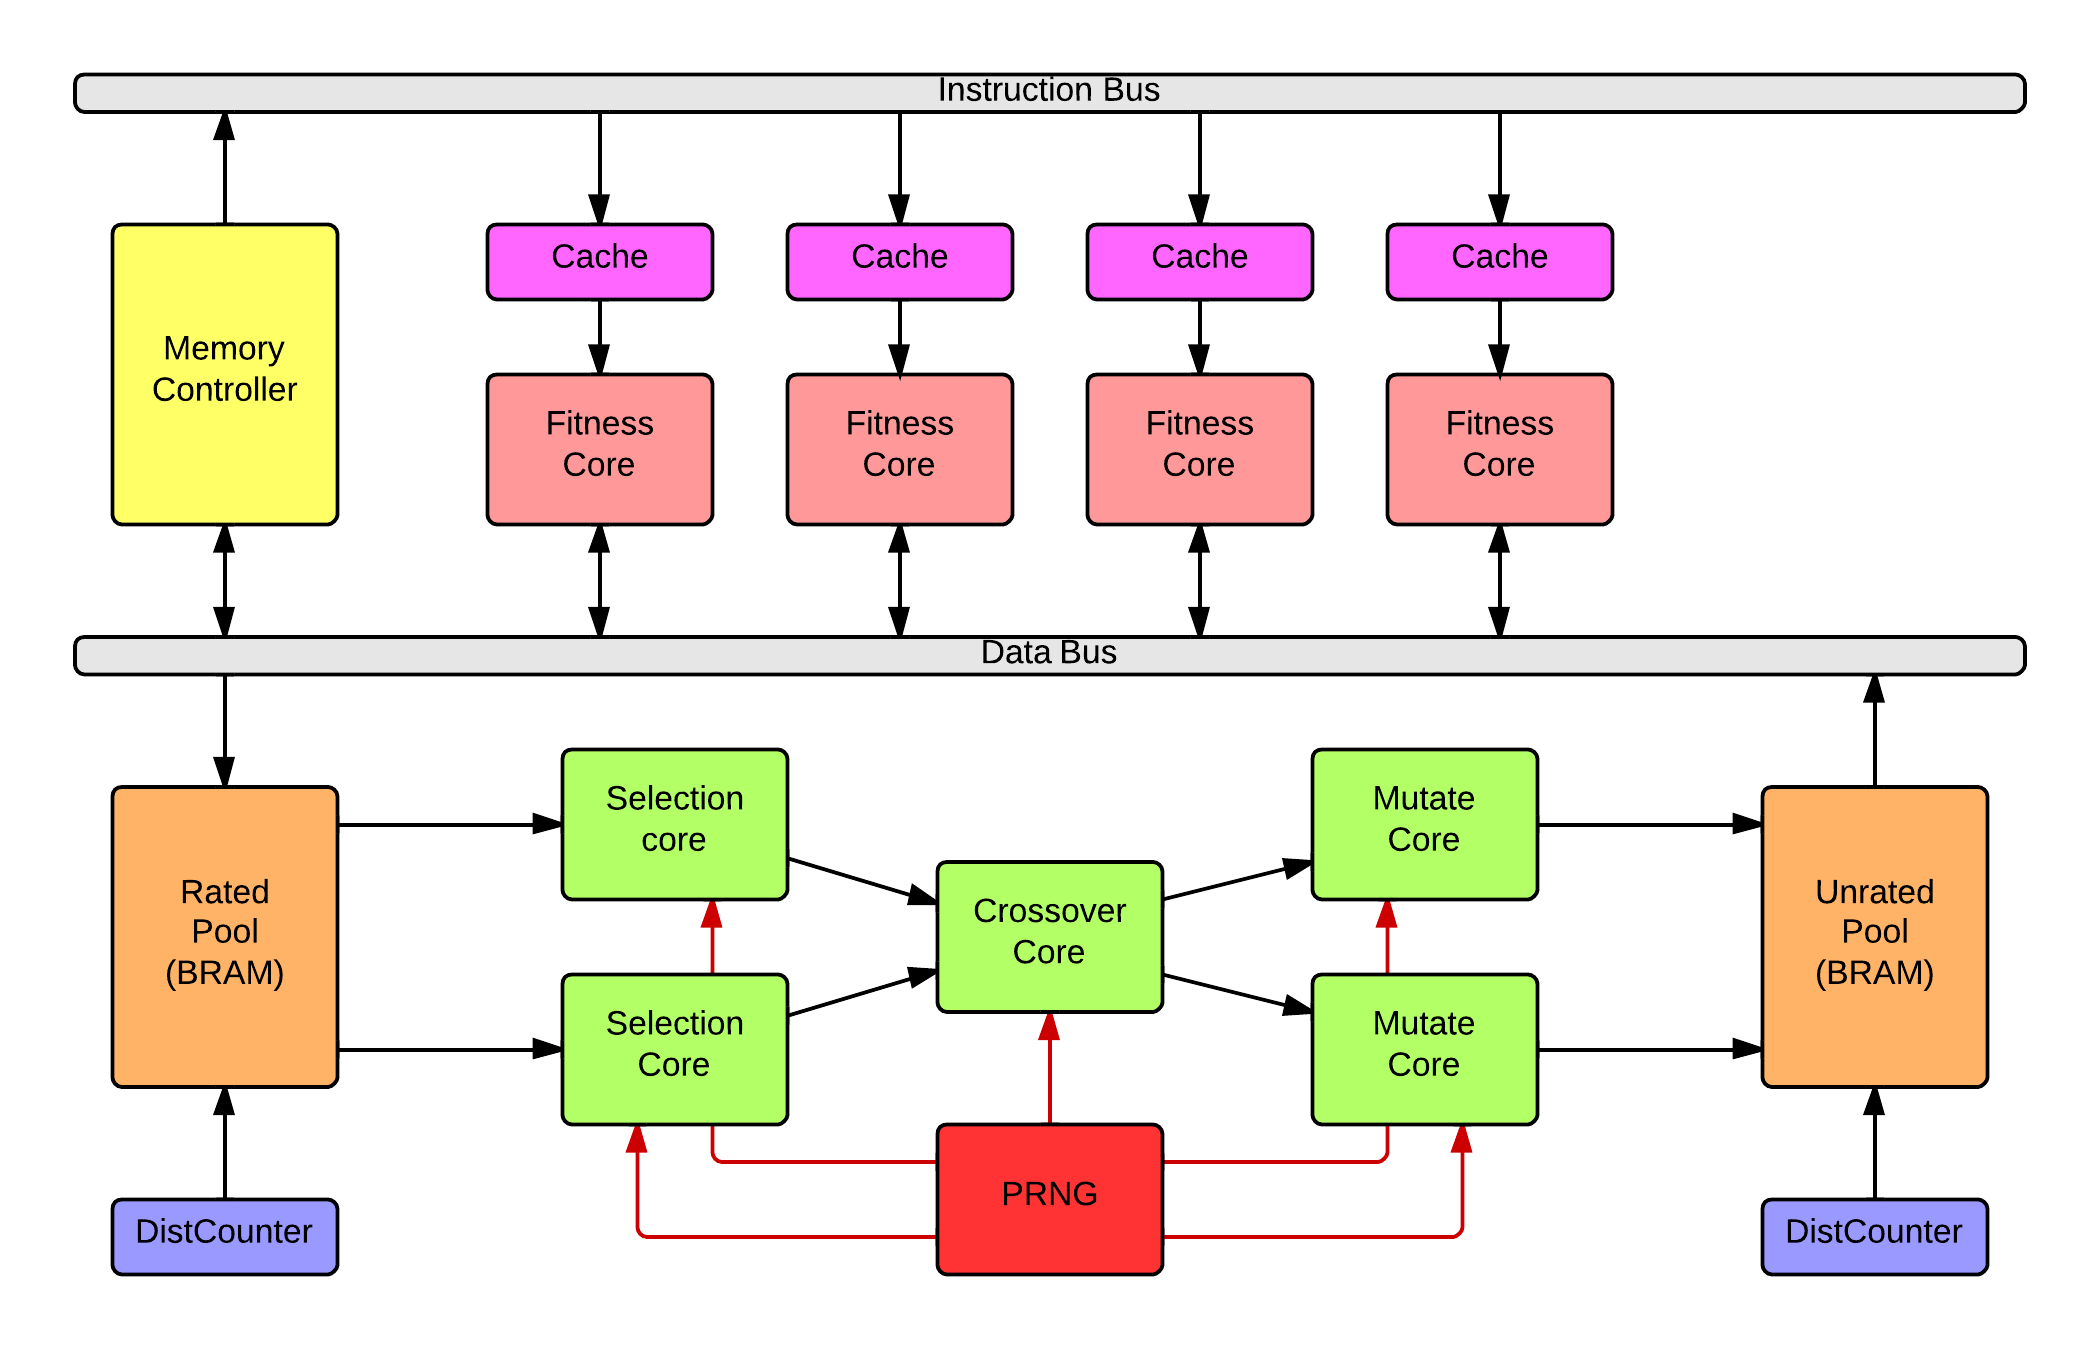
\includegraphics[width=\textwidth]{fpga/fig/processor_architecture.png}
\caption{The figure shows the final processor architecture. Most of the figures seen in this picture as for instance "fitness core", are abstractions of more complex logic at lower levels (mostly MSI and LSI components). }
\label{figure:fpga-architecture}
\end{figure}

\todo{Modify figure \vref{figure:fpga-architecture} so that it is easy to see that the number of fitness cores is configurable.}

The processor architecture designed for the Barricelli computer is a very clean design, and the key to its high performance lies in its simplicity.
The architecture contains a number of general cores, which in this context are named fitness cores.
The fitness cores are general purpose cores in the sense that they are programmable and turing complete, but for genetic algorithm applications the cores are intended to calculate fitness scores of individuals.

The number of fitness cores is configurable.
The reference implementation of the Barricelli computer is configured to have 7 fitness cores.

Common genetic algorithms operations are performed by a separate hardware accelerator pipeline.
This accelerator consists of several operation-specific special cores for selection, crossover and mutation.
The fitness cores and the genetic pipeline are all connected to a single data bus.
To avoid any memory synchronization issues the data bus is controlled by a central arbitration unit.

The processor architecture is illustrated in figure \vref{figure:fpga-architecture}.


\subsection{Instruction Memory}
\label{subsec:fpga-instruction-memory}
The \Gls{barricelli} is a \Gls{harvard machine}.
The memory is split into instruction and data memory.
This is done to achieve better memory throughput, because both memories can be accessed simultaneously.
The instruction memory is organized in a two layer memory hierarchy, with slower external memory (\gls{SRAM}) and faster, internal on-chip caches (\gls{BRAM}).
This separation combines the high instruction thoughput of fast on-board memory wit the comfortably spaceous data storage capabilities of a larger, slower chip external chip.

Each fitness core has its own private instruction memory cache which buffers instructions to decrease the number of slow memory accesses needed during runtime.
Access to an instruction cache is handled by a fitness core's dedicated cache controller, which is responsible for locating and transferring instructions from the instruction memory.
In case of a cache miss, the data-requesting core is halted until the instruction is transferred from memory.
A pseudo-algorithm describing the cache fetch operation can be found in algorithm \vref{algorithm:cache-operation}.
This scheme is created to resolve the conflicts that arise from using shared memory. 

\begin{algorithm}[H]
\SetAlgoLined
\DontPrintSemicolon
\KwData{ $ a = $ an instruction address \newline
$ Ci = $ an array of instructions \newline
$ Ca = $ an array of the corresponding addresses \newline
$ M = $ the instruction memory, indexable by instruction addresses
}
\KwResult{The instruction at address $ a $}
\Begin{
    \If{$ a = Ca[A \bmod{512}] $}{
        \Return{$ Ci[A \bmod{512}] $}
    }\Else{
        $ Caa \bmod{512}] \longleftarrow a $\;
        $ Ci[a \bmod{512}] \longleftarrow M[a] $\;
        \Return{$ Ci[A \bmod{512}] $}
    }
}
\caption{Fetching an instruction from the cache}
\label{algorithm:cache-operation}
\end{algorithm}


\subsection{Data Memory}
\label{subsec:fpga-data-memory}
The \gls{galapagos} architecture is a \gls{MIMD} architecture with shared memory.
In the \Gls{barricelli} computer, a central memory controller is responsible for synchronizing memory access on the shared data bus.
Each component that wants to access memory must go through the memory controller, and follow the proper memory access request protocol.
The controller is constructed in a way that only allows one fitness core to be able to carry out a memory request at a single time.
In case of multiple memory requests, the controller performs a selection deciding in which order the requesting cores is granted the bus.
The precise technique of selection can be seen in algorithm \ref{algorithm:round-robin-selection}.
This may introduce a potential bottleneck for memory-bound problems.
For this reason, each fitness core has a generous 31 general purpose registers, which should reduce the data memory load quite a bit.

\begin{figure}[H]
\begin{algorithm}[H]
\SetAlgoLined
\DontPrintSemicolon
\KwData{$ Requests = $ requests signals from the fitness cores\newline 
$ Request = $ 2-bits specifying the operation}
\Begin{
    $ Requests \longleftarrow $ requests from the fitness cores\;
    \While{$ True $}{
        \For {request in Requests} {
            \If{request $=$ asserted}{
                performMemoryOperation()
            }
        }
        
    }
}
\caption{Round-robin selection}
\label{algorithm:round-robin-selection}
\end{algorithm}
\end{figure}


The selection algorithm is based on round-robin scheduling, and will be explained in further detail here.
The request signals of \emph{fitness cores} are checked in turn to check if one of the cores has requested the memory bus.
The type of request is determined by combination of two request signals sent by each \emph{fitness core}.
The signals refer to either a \emph{NOP}, \emph{READ}, or \emph{WRITE} operation.
In case of \emph{NOP}, the algorithm moves on to check the next state request lines.
It continues doing this in this fashion until a \emph{READ} or \emph{WRITE} request is encountered. 

When a \emph{READ} or \emph{WRITE} operation is encountered, the \emph{data controller} starts to carry out the request from the fitness core.
Performing a memory operation takes at least four cycles, as the processor word size is 64 bits, while the memory bus to the external memory chips are only 16 bits wide.
Because of this, data needs to be shuffled across the bus 16-bits at a time, which accounts for the four cycle minimum for data operations.

For the external memory to be operated correctly by the memory controller, the proper control signals need to be set at the correct times. The signals required differs depending on the type of operation, \emph{READ} or \emph{WRITE}. The timing diagrams can be seen in figure \ref{fpga:fig:timing:dmem:read} and \ref{fpga:fig:timing:dmem:write}, respectively. 

\todo{Check text}

\begin{figure}[H]
  \centering
  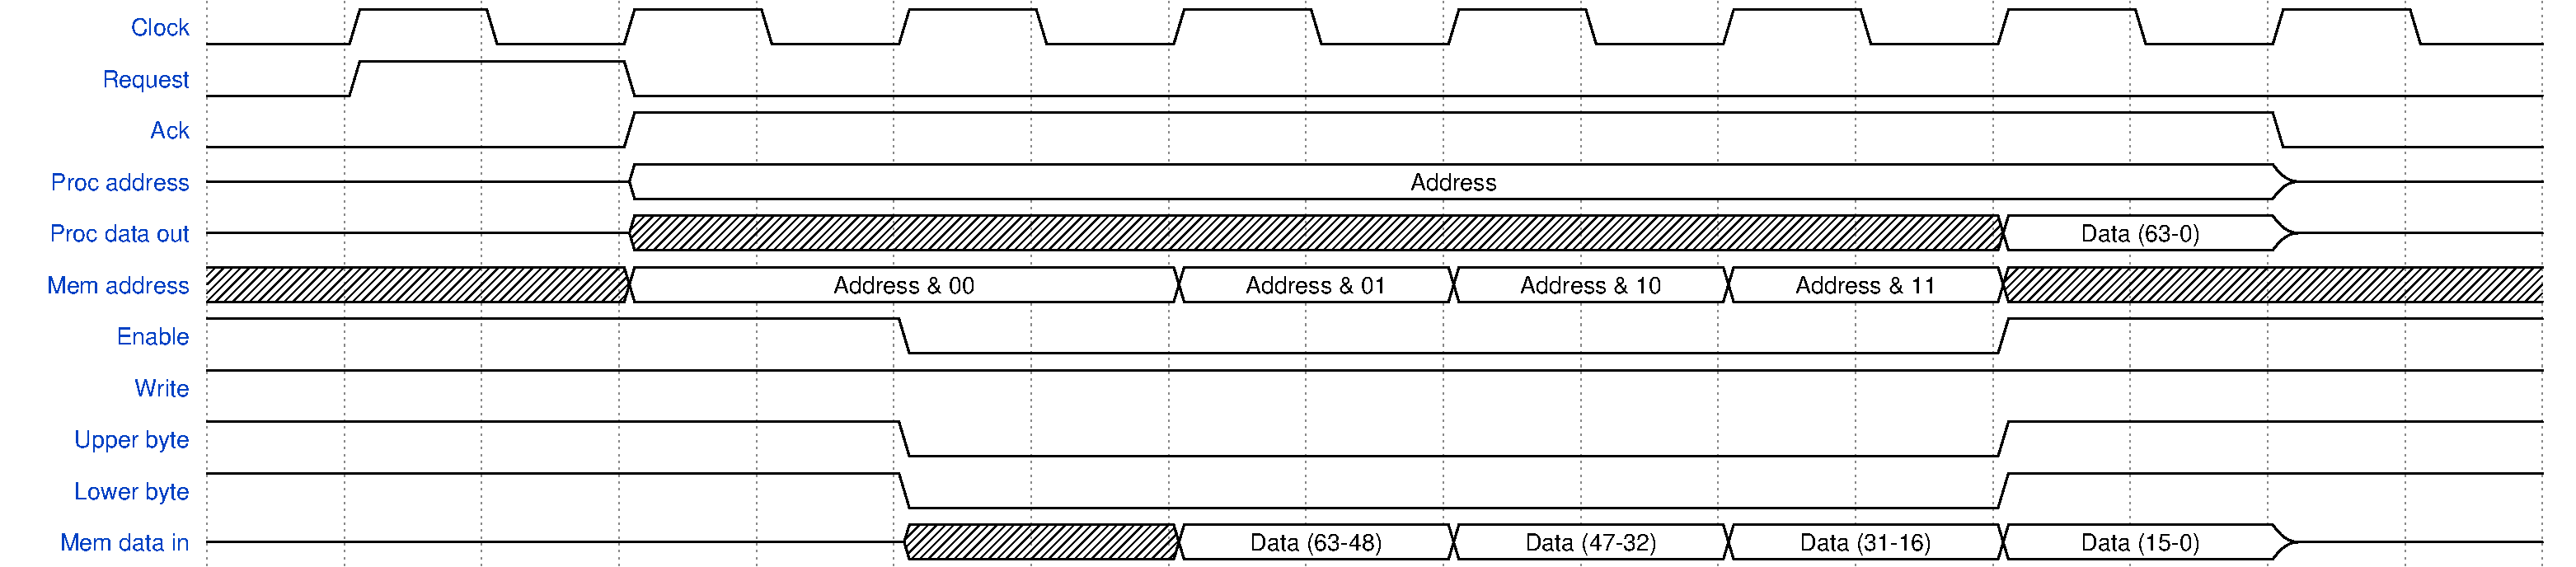
\includegraphics[width=\textwidth]{fpga/fig/timing/data_mem_read.pdf}
  \caption{Data memory read cycle}
  \label{fpga:fig:timing:dmem:read}
\end{figure}

\begin{figure}[H]
  \centering
  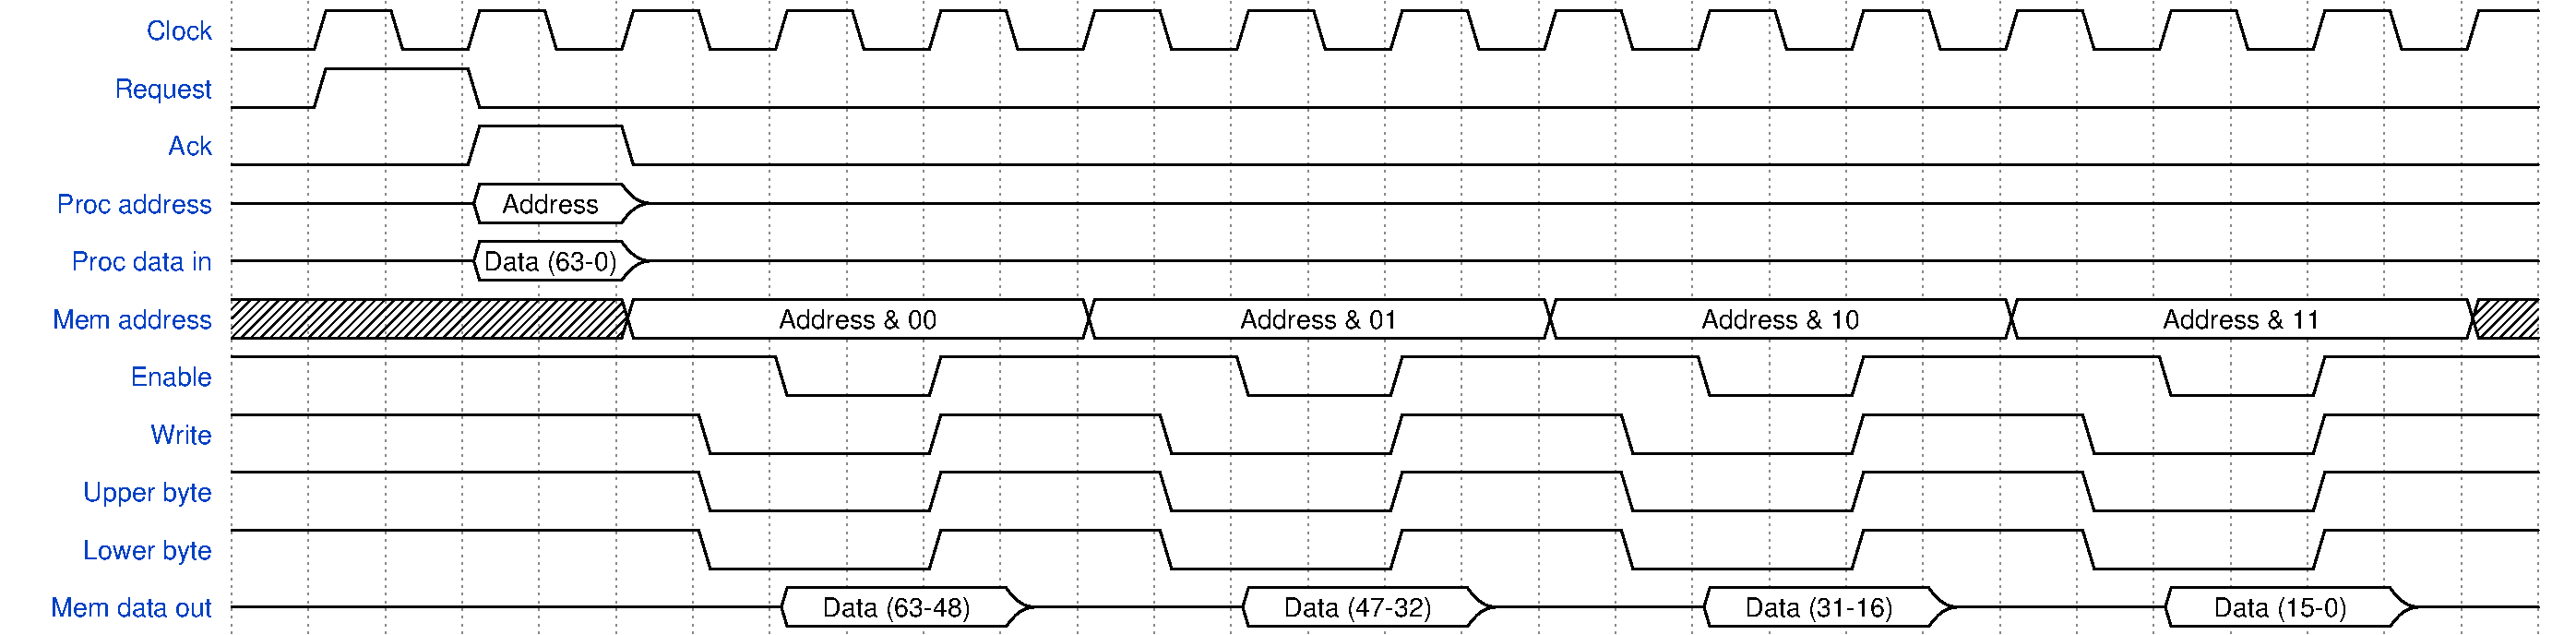
\includegraphics[width=\textwidth]{fpga/fig/timing/data_mem_write.pdf}
  \caption{Data memory write cycle}
  \label{fpga:fig:timing:dmem:write}
\end{figure}

As is immediately apparent in figures \vref{fpga:fig:timing:dmem:read} and \vref{fpga:fig:timing:dmem:write}, the number of cycles required for load and store operations are are 5 and 13 cycles, respectively.
A state machine is implemented in the \emph{data memory controller} to handle interfacing with the external memory chips.
This state machine is responsible for controlling that the different signals are set according to the diagrams.
For more detailed view of the \emph{Data memory controller}, the reader is advised to study the state machine diagram in figure \ref{fpga:fig:mem:data_memory_ctrl_state_machine} and the accompanying data path in figure \ref{fpga:fig:mem:data_memory_ctrl}.

\begin{figure}[H]
  \centering
  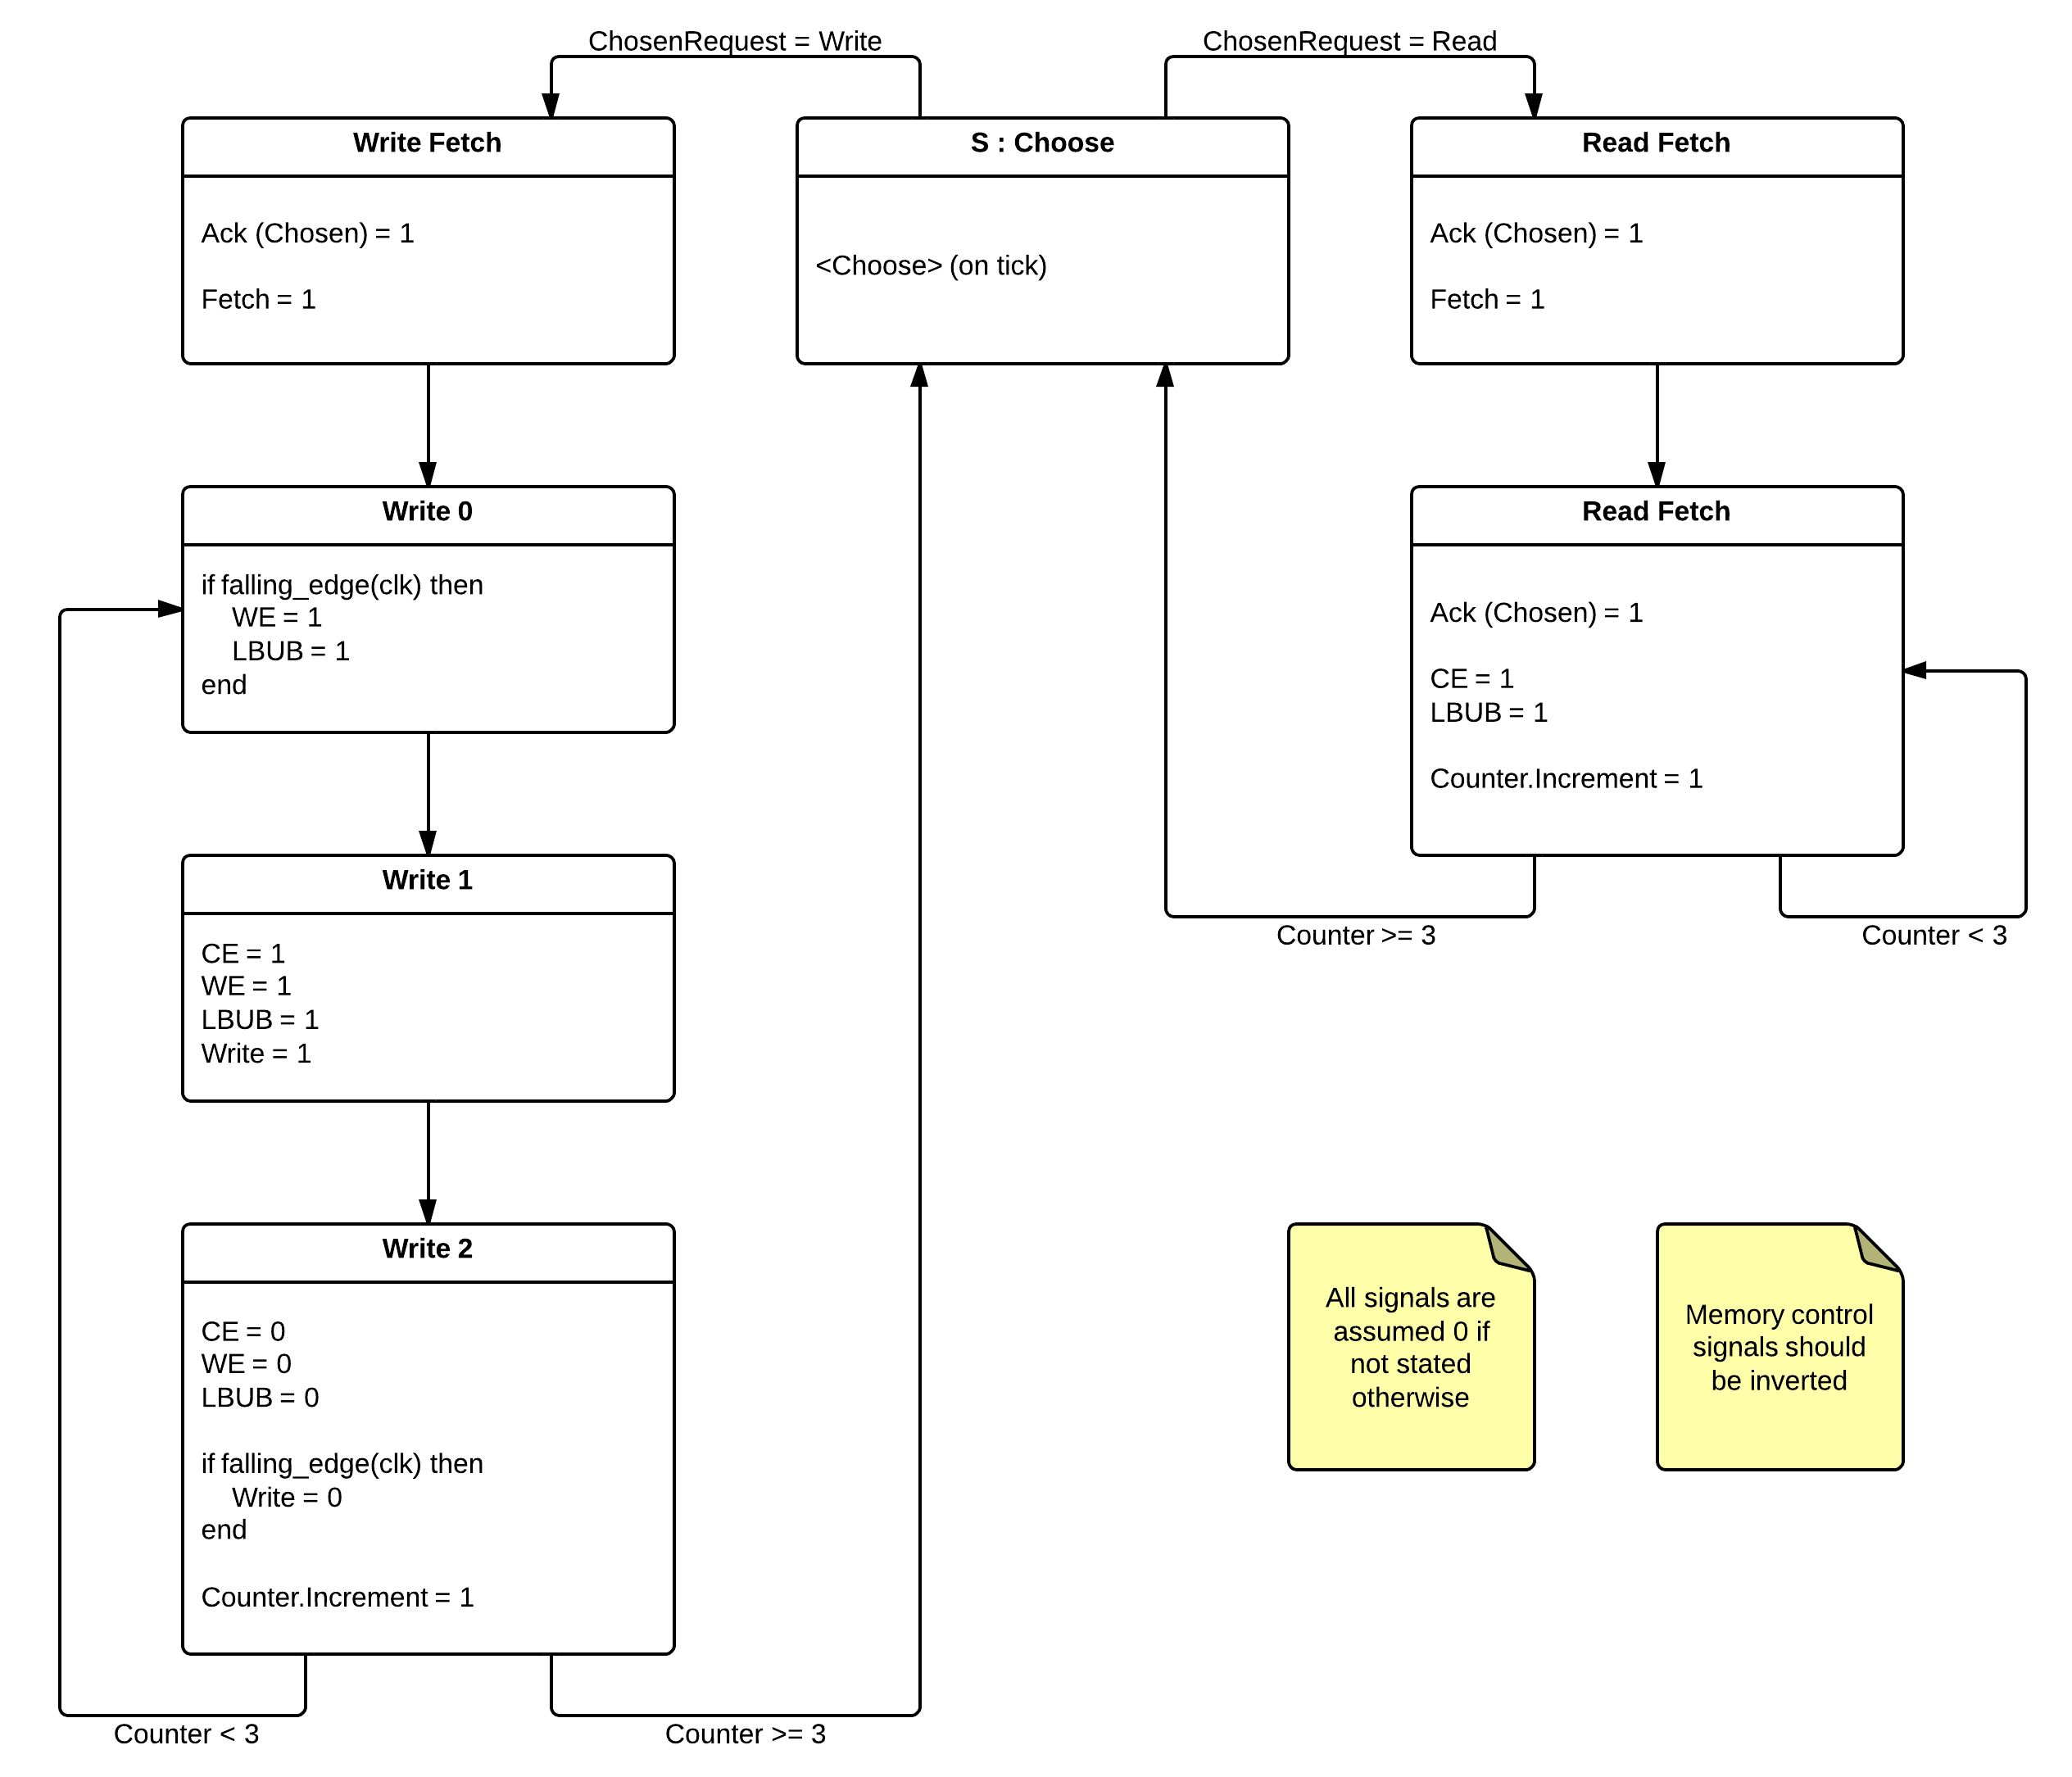
\includegraphics[width=\textwidth]{fpga/fig/memory_ctrl_state_machine.png}
  \caption{Data memory controller state machine}
  \label{fpga:fig:mem:data_memory_ctrl_state_machine}
\end{figure}


\begin{figure}[H]
  \centering
  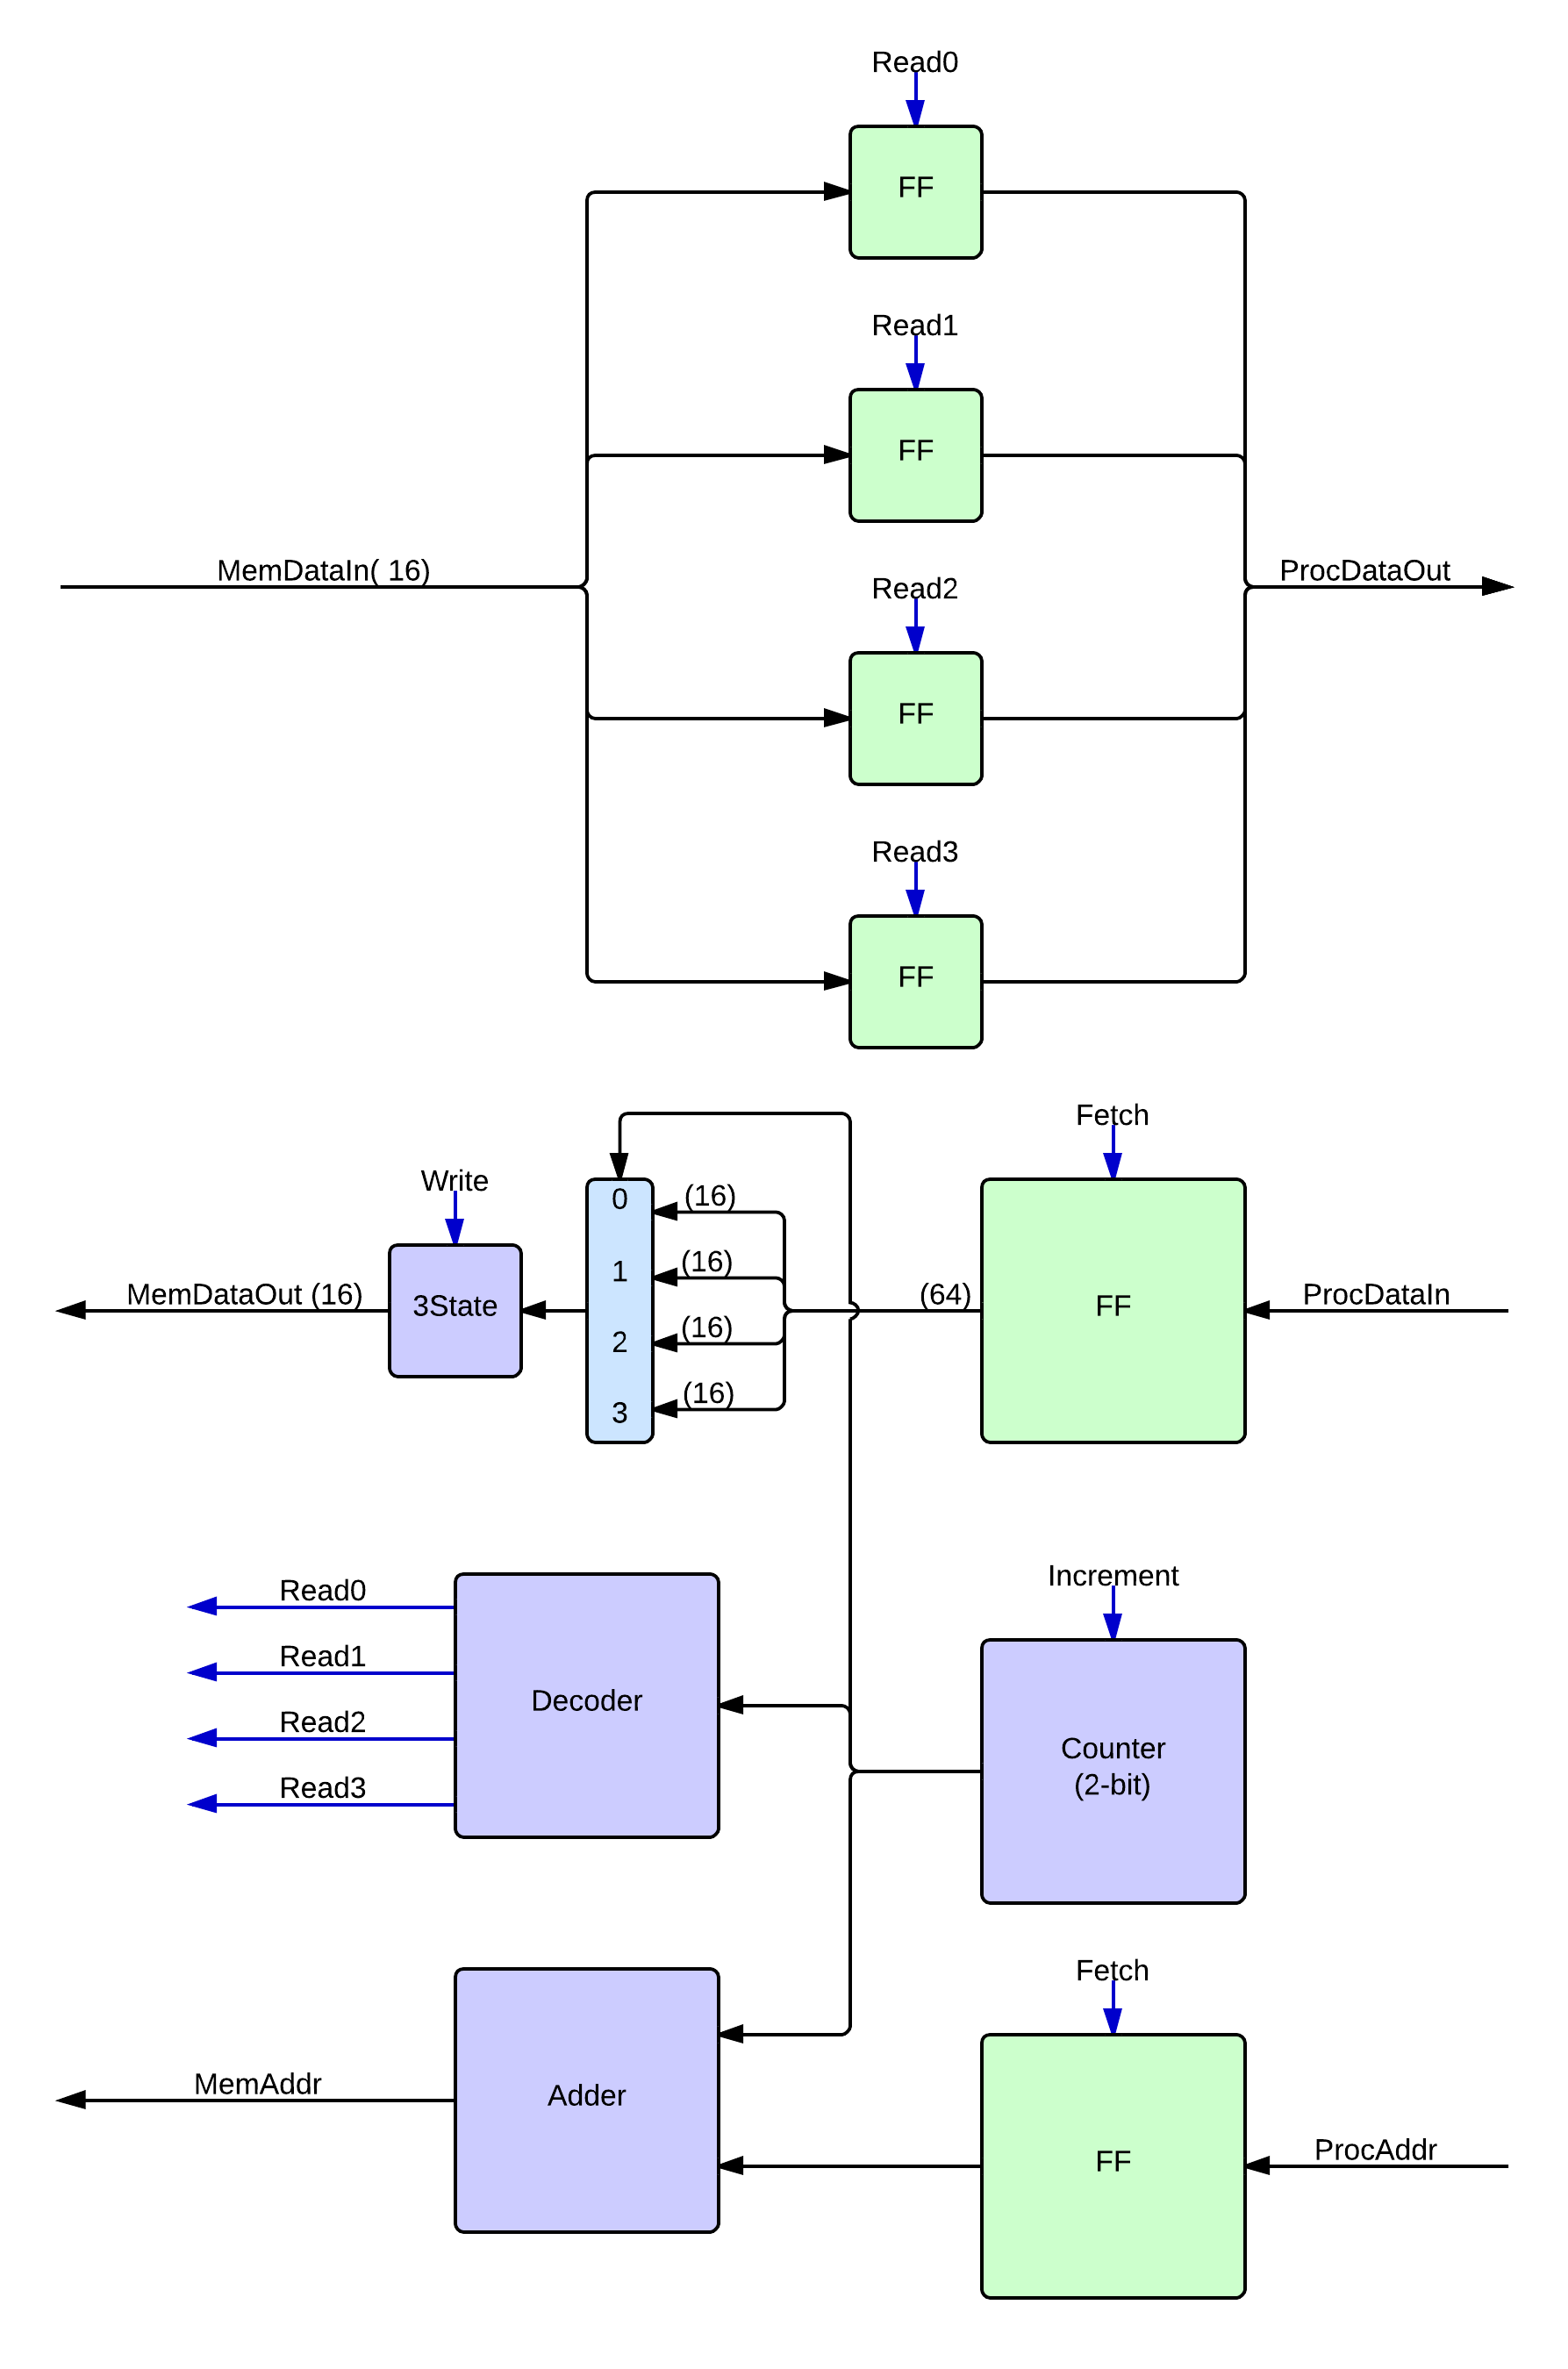
\includegraphics[width=\textwidth]{fpga/fig/memory_ctrl.png}
  \caption{Data memory controller signals mapping}
  \label{fpga:fig:mem:data_memory_ctrl}
\end{figure}


\todo{write about and ref to above graphs}


\subsection{Rated and Unrated Pools}
Individuals making up the populations are stored on the FPGA for for faster access. These are stored in \emph{BRAM} on the FPGA. This implies a lot faster access times, compared to access times to the external memory, as mentioned in (?). This is done to achieve better memory throughput when executing the algorithms. The pools are further divided into two separate \emph{BRAM} blocks, one for rated individuals, and one for un-rated. This is done to achieve even better memory throughput. The increased throughput are achieved because the different computational can work on the rated and un-rated pool simultaneously. For instance while one fitness core is storing a ranked individual, while another fitness core is fetching a new individual for ranking. 

\todo{More details and better explanation} 

Both the rated pool and the unrated pool is associated with the a controller, referred as the \emph{Genetic controller}. As with the data controller, this controller is responsible for granting access for the rated and unrated pool. This buses in question are, however, not the same as those used to access the data memory. The genetic controller use their own separate buses. The controller is based on mostly the same idea as the data controller described in section (?). The when performing genetic operations, the fitness cores need to request the data bus by using two request signals. The combination of these signals refer to the operation the fitness core requests from the genetic controller. 

The genetic cores continuously performs a round-robin in order to grant bus to the requesting fitness core. The logic surrounding the different operations are implemented as an state machine to divide the operations in different clock cycles. This is the same method as used in the data controller.







The state machine can be seen in figure(?)




\subsection{PRNG Module}
The genetic algorithms need diversity in the search space in order to be able to converge to a solution. To achieve this, the architecture need some way of creating sufficiently random numbers. These generated numbers do not need to be true randoms number, this implies that a psudo number generator will suffice. 

    
 

\subsection{Fitness Core} \label{fpga:fitness:ss:design_of_the_fitness_core}
    \subsection{Design of fitness core}

The design of the fitness core is highly influenced by MIPS.
The core is designed as a five stage pipeline.
The goal is to make it as simple as possible, and at the same time harvest efficiency by instruction level parallelism.
The more advanced features like branch prediction and instruction scheduling are not taken into consideration while designing the CPU.
The hazard detection schemes will be made simple.
The hazard resolutions will be made in software as well as in hardware.
The plan is to simply stall when we encounter any hazards in the pipeline.
The assembler will handle the most obvious ones to achieve efficiency, while the hardware will simply stall when hazards are detected.

\fxnote {The hazard scheme may change if time}
 \label{fpga:subsection:fitness_core}


\subsection{The Genetic Pipeline}
\label{fpga:subsection:genetic_pipeline}
\todo{some words about the genetics accelerator}
The galapagos architecture includes a highly specialised pipeline for performing genetic operations. The pipeline is based on the observation that selection, crossover, and mutation works similar for a specific subset of problems. These can therefore be implemented as hardware accelerators constructed for performing one specific task. Constructing such accelerators has been proven to be very beneficial regarding performance. Designing specialised hardware is usually simpler and thereby more effective than constructing general purpose components.\todo{Bullshit ?} This pipeline will effectively relieve the general cores, the fitness cores, from computing the evolution of individuals. The idea is that these will make the fitness cores able to only focus on the computation of fitness ranking, which is considered computational intensive. In the mean time the \emph{genetic pipeline} can produce new data for ranking. These operations could have been performed by the processor, however, the processor is badly suited for these kind of operations. Note that the instructions in the pipeline actually uses 5 cycles in order to complete propagate through the pipeline. It is a far better to only use one cycle in order to complete the one specific operation.  

The genetic pipeline is constructed with three specialised cores for performing selection, crossover, and mutation. These are operations that occurs frequently in genetic algorithms. These are connected to two internal memory banks on the \emph{FPGA}, namely the unrated and rated pool.


-Abstraction for the programmer. Simpler to program.
-Do not need components like ALU
- effective 
- Less control over the genetic pipeline
- 



\subsubsection {Selection Core} \label{fpga:selection:ss:selection_core}
    \input{fpga/selection-core} \label{fpga:subsection:selection_core}

\subsubsection{Crossover Core} \label{fpga:crossover:ss:crossover_core}
    \input{fpga/crossover-core} \label{fpga:subsection:crossover_core}

\subsubsection{Mutation Core}\label{fpga:mutation:ss:mutation_core}
    \input{fpga/mutation-core} \label{fpga:subsection:mutation_core}




\subsection{Parallelism}
\todo{awkwardly placed section.. move it somewhere else?}
The Barricelli is a MIMD computer, which means that it can execute multiple different instruction streams on multiple different data streams simultaneously, in parallel.
The four\cn fitness cores in the archtecture have each their own program counters and may load different data independantly of eachother.
They all share the same data and instruction memory, however, which makes the Barricelli a shared memory model MIMD computer.
Additionally, the genetic pipeline contains multiple specialized cores, which can also execute independant, less general instruction streams on independant data.

 \label{fpga:section:cpu_architecture}

%%Fitness core subsection
\subsection{Design of fitness core}

The design of the fitness core is highly influenced by MIPS.
The core is designed as a five stage pipeline.
The goal is to make it as simple as possible, and at the same time harvest efficiency by instruction level parallelism.
The more advanced features like branch prediction and instruction scheduling are not taken into consideration while designing the CPU.
The hazard detection schemes will be made simple.
The hazard resolutions will be made in software as well as in hardware.
The plan is to simply stall when we encounter any hazards in the pipeline.
The assembler will handle the most obvious ones to achieve efficiency, while the hardware will simply stall when hazards are detected.

\fxnote {The hazard scheme may change if time}
 \label{fpga:subsection:fitness_core}

%%Selection core subsection
\subsection {Design of the selection core} \label{fpga:selection:ss:selection_core}

The selection core is designed based on a tournament selection algorithm. It is designed to select an chromosome from a random position in the rated pool. The current best and the random selected is compared to each other with use of an comparator. The best chromosome is stored and used in the next tournament round. After some number of tournaments the current best is transferred to the crossover core. The selection core is actually responsible for letting the rest of the genetic pipeline know when it can fetch the next chromosome. 

The selection core is designed with efficiency in mind. The overall time spent in the genetic pipeline must be smaller than the time spent ranking the chromosomes. Note that the fitness cores are connected to the same memory bus as the genetic pipeline. This could potentially lead to a memory bottleneck resulting in starvation. The selection core tries to overcome this fact by reducing the memory access to a minimum. Note that the selection core has reserved the memory bus during the ongoing tournament. This implies that port used by the selection core is unavailable to others during this time. It is designed to not use the memory more than it absolutely have to. For instance, if the current fitness value is greater than the fitness value just fetched. The selection core will not bother fetching the accompanying chromosome. Ensuring that the memory resources are not wasted. This is accomplished with an \emph{state machine}. 



\subsubsection{Data Path}
Upon the beginning of the data path design, the group wanted to determine the the components required to perform the selection. In this specific case the group decided to design a data path able to perform a tournament selection. The resulting architecture is made as simple as possible.  It is composed of \emph{flip flops}, \emph{control unit} and an \emph{comparator}. The different components are connected as seen in figure.




\fxnote{Add figure of selection core}


\subsubsection{Control Unit} \label{fpga:selection:sss:control_unit}



\subsubsection {Comparator} \label{fpga:selection:sss:comparator}



\subsubsection{Case study} \label{fpga:selection:sss:case_study}



 \label{fpga:subsection:selection_core}

%%Crossover core subsection
The crossover Core is the next part in the genetics accelerator after the selection cores. Two inputs are forwarded from the two selections cores as "parents", and two outputs are the "children" of the inputs, containing bits from both parents. All the bits from both the parents are forwarded in the children, but in some parts the bit-patterns are switched on the children, based a selected crossover function and on a random input from the PRNG. Henceforth this is called crossover.

There are three distinct crossover functions that are implented: Split, doublesplit and function.

\paragraph{\textit{Split Fucntion}}
\begin{figure}[H]
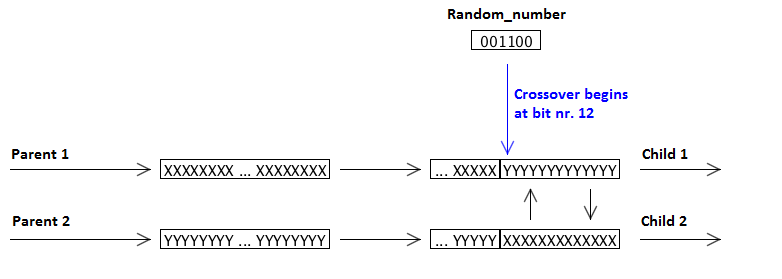
\includegraphics[width=\textwidth]{fpga/fig/crossover_split.png}
\caption{Crossover split function}
\label{fig_crossover_split}
\end{figure}

The first function, crossover split, performs crossover from a selected bit number in the children and until the edge (bit number 0). This can be seen in figure \ref{fig_crossover_split}. The values in the parents are represented with X's and Y's, and a single X or Y can have the value 0 or 1, independent of each other.
The bit number for starting crossover is based on the value of a 6-bit input random\_number, which is provided by the PRNG. This value ranges from 0 to 63.

\todo Describe how it technically works??

\paragraph{\textit{Double-split Fucntion}}
\begin{figure}[H]
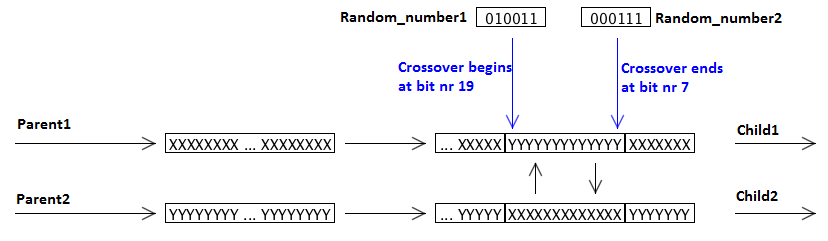
\includegraphics[width=\textwidth]{fpga/fig/crossover_doublesplit.png}
\caption{Crossover double-split function}
\label{fig_crossover_doublesplit}
\end{figure}

The second function, crossover double-split, is similar to the crossover\_split-function, but in additionally to having a starting bit for crossover, it also has an ending bit where the crossover starts, instead of reaching the edge at bit nr. 0. PRNG provides with 2 6-bit inputs, random\_number1 and random\_number2, whose values selects the starting bit and the ending bit for the crossover. These values range from 0 to 63, and if both are the same, then only one bit will be selected for crossover.

\todo Describe how it technically works??

\paragraph{\textit{XOR Fucntion}}
\begin{figure}[H]
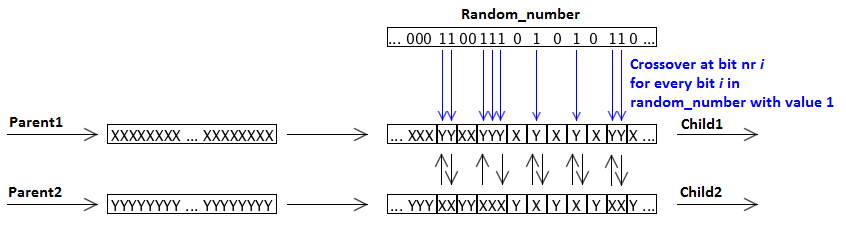
\includegraphics[width=\textwidth]{fpga/fig/crossover_xor.png}
\caption{Crossover XOR function}
\label{fig_crossover_xor}
\end{figure}

The third function, crossover XOR, performs crossover bit by bit, based on the 64-bit input random\_number. For each bit number \textit{i} in random\_number that has the value 1, the function will perform crossover on the children at the same bit number \textit{i}. This function is called XOR because of use of XOR-gates in earlier version of the function, and the principle is still the same: For each bit number \textit{i} in the child, the value will the bit number \textit{i} from one and only one parent. And which parent it is depends on the value of bit number \textit{i} in random\_number.

\todo Describe how it technically works??

\paragraph{\textit{Crossover Core Toplevel}}

The crossover core is implemented on the genetics accelerator as a toplevel containing 3 subcores, one for each function, as well as a fourth path with no crossover. In addition to the two parent inputs and 64-bit input random\_number, the toplevel has a control\_number input used for determining which crossover function is to be used: Split, doublesplit, xor, "party mode" or no crossover at all. Party mode is choosing crossover function at random, based on the 2 LS bits in the random\_number. In this way, whenever inputs are sent through the crossover\_toplevel, different functions may be used at different times. These are the control values:
\begin{itemize}
\item 000 - Split
\item 001 - Double-split
\item 010 - XOR
\item 011 - No crossover
\item 1XX - Party mode, in which case these are the random control values:
    \begin{itemize}
    \item 00 - Split
    \item 01 - Doublesplit
    \item 10 - XOR
    \item 11 - No crossover
    \end{itemize}
\end{itemize} \label{fpga:subsection:crossover_core}

%%Mutation core subsection
The mutation core is the final part in the genetics accelerator. The mutation core takes in a forwarded child from the crossover core as input and may perform mutation on a few selected bits before passing on the result. 

\begin{figure}[H]
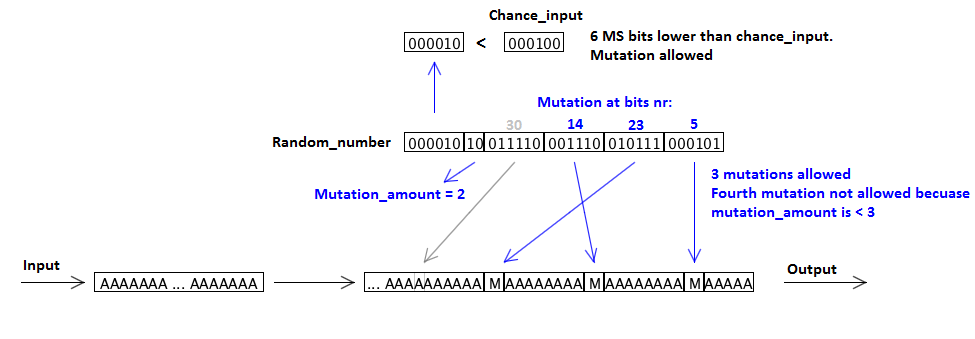
\includegraphics[width=\textwidth]{fpga/fig/mutation.png}
\caption{Mutation core function concept}
\label{Fig_Mutation}
\end{figure}

In addition to the the 64-bit child, the mutation core also takes in a 32-bit random\_number and a 6-bit chance\_input as inputs. As it can be seen in the example in figure \ref{Fig_Mutation}, all bits that are not mutated are represented by an A, and mutated bits are represented with M. The values in each A or M can be 0 or 1, independent of each other. The value M at bit number \emph{i} is the opposite of the original value A at same bit number \emph{i} in the input.
The 6 first bits in the random\_number is compared to the chance\_input, and mutation happens only if the value of these bits are less than the chance input. For each different value in chance\_input, the user may increase or decrease the chance of mutation by about 1,5\%, or $(1 / 2^6)$. If the chance input is set to 000000, no mutation will ever happen, and the user may in this way disable the mutation core.

The next two bits in the random number (bits 25-24) are used to determine how many mutations will happen. There are 4 different values, therefore there can be 1-4 mutations.
The next 24 bits are used to determine which bits are to be mutated. 6 bits are used for finding each bit number. This is similar to what is done in the split and doublesplit functions in the crossover core. These values are numbered, representing their bit field:
\begin{itemize}
\item Nr. 1: 5-0
\item Nr. 2: 11-6
\item Nr. 3: 17-12
\item Nr. 4: 23-18
\end{itemize}
These are numbered after the amount of allowed mutation. Nr. 1 will always happen when a mutation occurs, while nr. 4 happens only when the amount\_number allows for 4 mutations.

Note that if more than one of these numbers point to the same bit to be mutated, the output M will still be the inverted from the original input. For instance, if both numbers 1 and 2 (bits 11-6 and 5-0) have the value 000110, and therefore point at bit number 6, the same mutation will still happen as if only one of these numbers were 000110. If the input bit was 1, the mutated will be 0, and vice versa.
In the example provided in figure \ref{Fig_Mutation}, the 6 first bits of the random\_number are less than the chance\_input, therefore a mutation happens. Bits 23-0 have the values 30, 14, 23 and 5. Because the value of bits 25-24 is 10 (mutation\_amount has value 2), there will be 3 mutations, and the fourth does not occur (though the figure shows where it would have occured if allowed).

\begin{figure}[H]
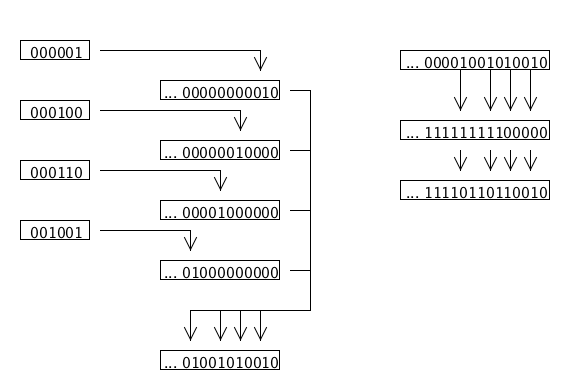
\includegraphics[width=\textwidth]{fpga/fig/mutation_mask.png}
\caption{Setting mutation}
\label{fig_mutation_mask}
\end{figure}

The mutation core is implemented by use of four shifter variables, one for each possible mutation, and set so that only one bit is 1 for the output. A final mutation is set by combining the outputs from the shifter variables by using OR-funftion, and the mutation\_amount determines how many of these outputs are combined. Figure \ref{fig_mutation_mask} shows an example where bits 1, 4, 6 and 9 are set for mutation. In this case the final output is set by combining the input and mutation with the XOR-fuction, so that for each bit \emph{i}, the bit is set to 1 if and only if bit \emph{i} is set in either the input or the mutation, but not both. This can be seen in figure \ref{fig_mutation_perform}.

\begin{figure}[H]
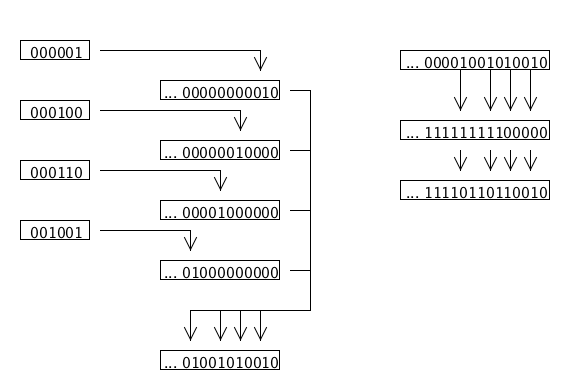
\includegraphics[width=\textwidth]{fpga/fig/mutation_mask.png}
\caption{Performing mutation}
\label{fig_mutation_perform}
\end{figure}

\todo{ "Selected bit number" needs to somehow be defined in the description of the shifter variable + ShifterVariable needs to be described.} \label{fpga:subsection:mutation_core}

#if 0
PCB
    Design Choices
        IO devices
        Internal Communication
        External communication
        Memory
    Power Supply
    Power Plane
    Footprints
        
    Process
        System design
        PCB design and routing
        Soldering
    Problems and workaround
#endif


\section{Processor Design (FPGA)}
	The Barricelli computer features a custom processor design.
The processor is a MIMD processor designed for high performance genetic algorithms computing.
This chapter describes the processor architecture and documents the design decisions made.

\section {Initial requirement}
    \section {Initial requirement}
The assignment require the development of MIMD CPU architecture.
One of the core requirement is to be able to run multiple instruction streams working on multiple data streams.
 \label{fpga:section:initial_requirements}
\subsection{Parallelism}

The Barricelli is a MIMD computer, which means that it can execute multiple different instruction streams on multiple different data streams simultaneously, in parallel.
The cores in the archtecture have each their own program counters and may load different data independantly of each other.
Several of the cores share the same data and instruction memory, however, which makes the Barricelli a shared memory model MIMD computer.



\section{Instruction Set Architecture} \label{fpga:isa:s:isa}
    The \Gls{galapagos} Instruction Set Architecture is the instruction set archtecture designed for the \Gls{barricelli} computer for this project.
The architecture is loosely based on the well-known and tested \gls{MIPS} architecture, but borrows inspiration from many other different sources as well.
Especially inspirational for the design of the \Gls{galapagos} ISA have been the \gls{MIPS} core design principles, which can be found in table \vref{fpga:tbl:mips-design-principles}.

\begin{table}[H]
\centering
    \begin{tabular}{l l} 
     \textbf{Design principle 1} & Simplicity favours regularity.~\cite[p.~79]{compOrgDes}. \\
     \textbf{Design principle 2} & Smaller is faster.~\cite[p.~81]{compOrgDes} \\
     \textbf{Design principle 3} & Make the common case fast.~\cite[p.~86]{compOrgDes} \\
    \hline
\end{tabular}
    \caption{MIPS Design Principles}
    \label{fpga:tbl:mips-design-principles}
\end{table}

The Galapagos ISA was designed and fully specified quite early in the project, which made it an important resource for the rest of the component design process.

While the ISA is thoroughly documented in appendix \vref{appendix:isa}, the rest of this section will present a short overview for the reader's convenience.

\bigskip
\bigskip

The \Gls{galapagos} instruction set architecture is a RISC architecture.
The instructions are kept simple, and only perform very specific and small tasks.
That is, the instructions are low-level instructions executed directly in hardware without the need for additional decoding in form of microinstructions or the like.

\subsection{Instruction Formats}

As \Gls{MIPS}, \Gls{galapagos}, in true \gls{RISC} fashion, has relatively few instruction formats.
These instruction formats are constructed to be regular, which implies that the different information types contained in an instruction are always located in the same positions, when possible.
This makes the instruction decoding process in the processor much simpler.
This is done in accordance with design principle 1 of table \vref{fpga:tbl:mips-design-principles}.

The three instruction formats used in \Gls{galapagos} are the RRR, RRI and RI formats.
They are named after the types of data they contain.
RRR contains three register addresses.
RRI contains two register addresses and one immediate.
RI contains one register address and a larger immediate.

Every instruction has a set of conditional flags that may be set.
Through these flags, a programmer can decide whether or not an instruction will be executed.
This allows for branchless conditional execution of single instructions.
These conditional signals allow for many clever applications - a \gls{nop} instruction can be implemented as any instruction with the condition set to ``never execute''.
Indeed, even conditional branching is implemented as a branch-less conditional!
For a more detailed docummentation of the \gls{galapagos} instruction set architecture, the reader is encouraged to read appendix \vref{appendix:isa}.


\subsection{Genetics Instructions}

One of the requirements in section \vref{section:requirements} was that the ISA should support genetic-specific instructions to facilitate performant genetic algorithms programming.
Present in the \Gls{galapagos} ISA are the genetic instructions \texttt{ldg}, \texttt{stg} and \texttt{setg}.
They are the instructions for loading and storing \glspl{individual} to the genetics accelerator, and configuring the genetics accelerator, respectively.
With these instructions available to the programmer, using the genetics accelerator is easy and painless.
The reader may refer to the ISA documentation in appendix \vref{appendix:isa} for in-depth documentation about how the genetics instructions are used.



\section {Processor Architecture}
    \begin{figure}[H]
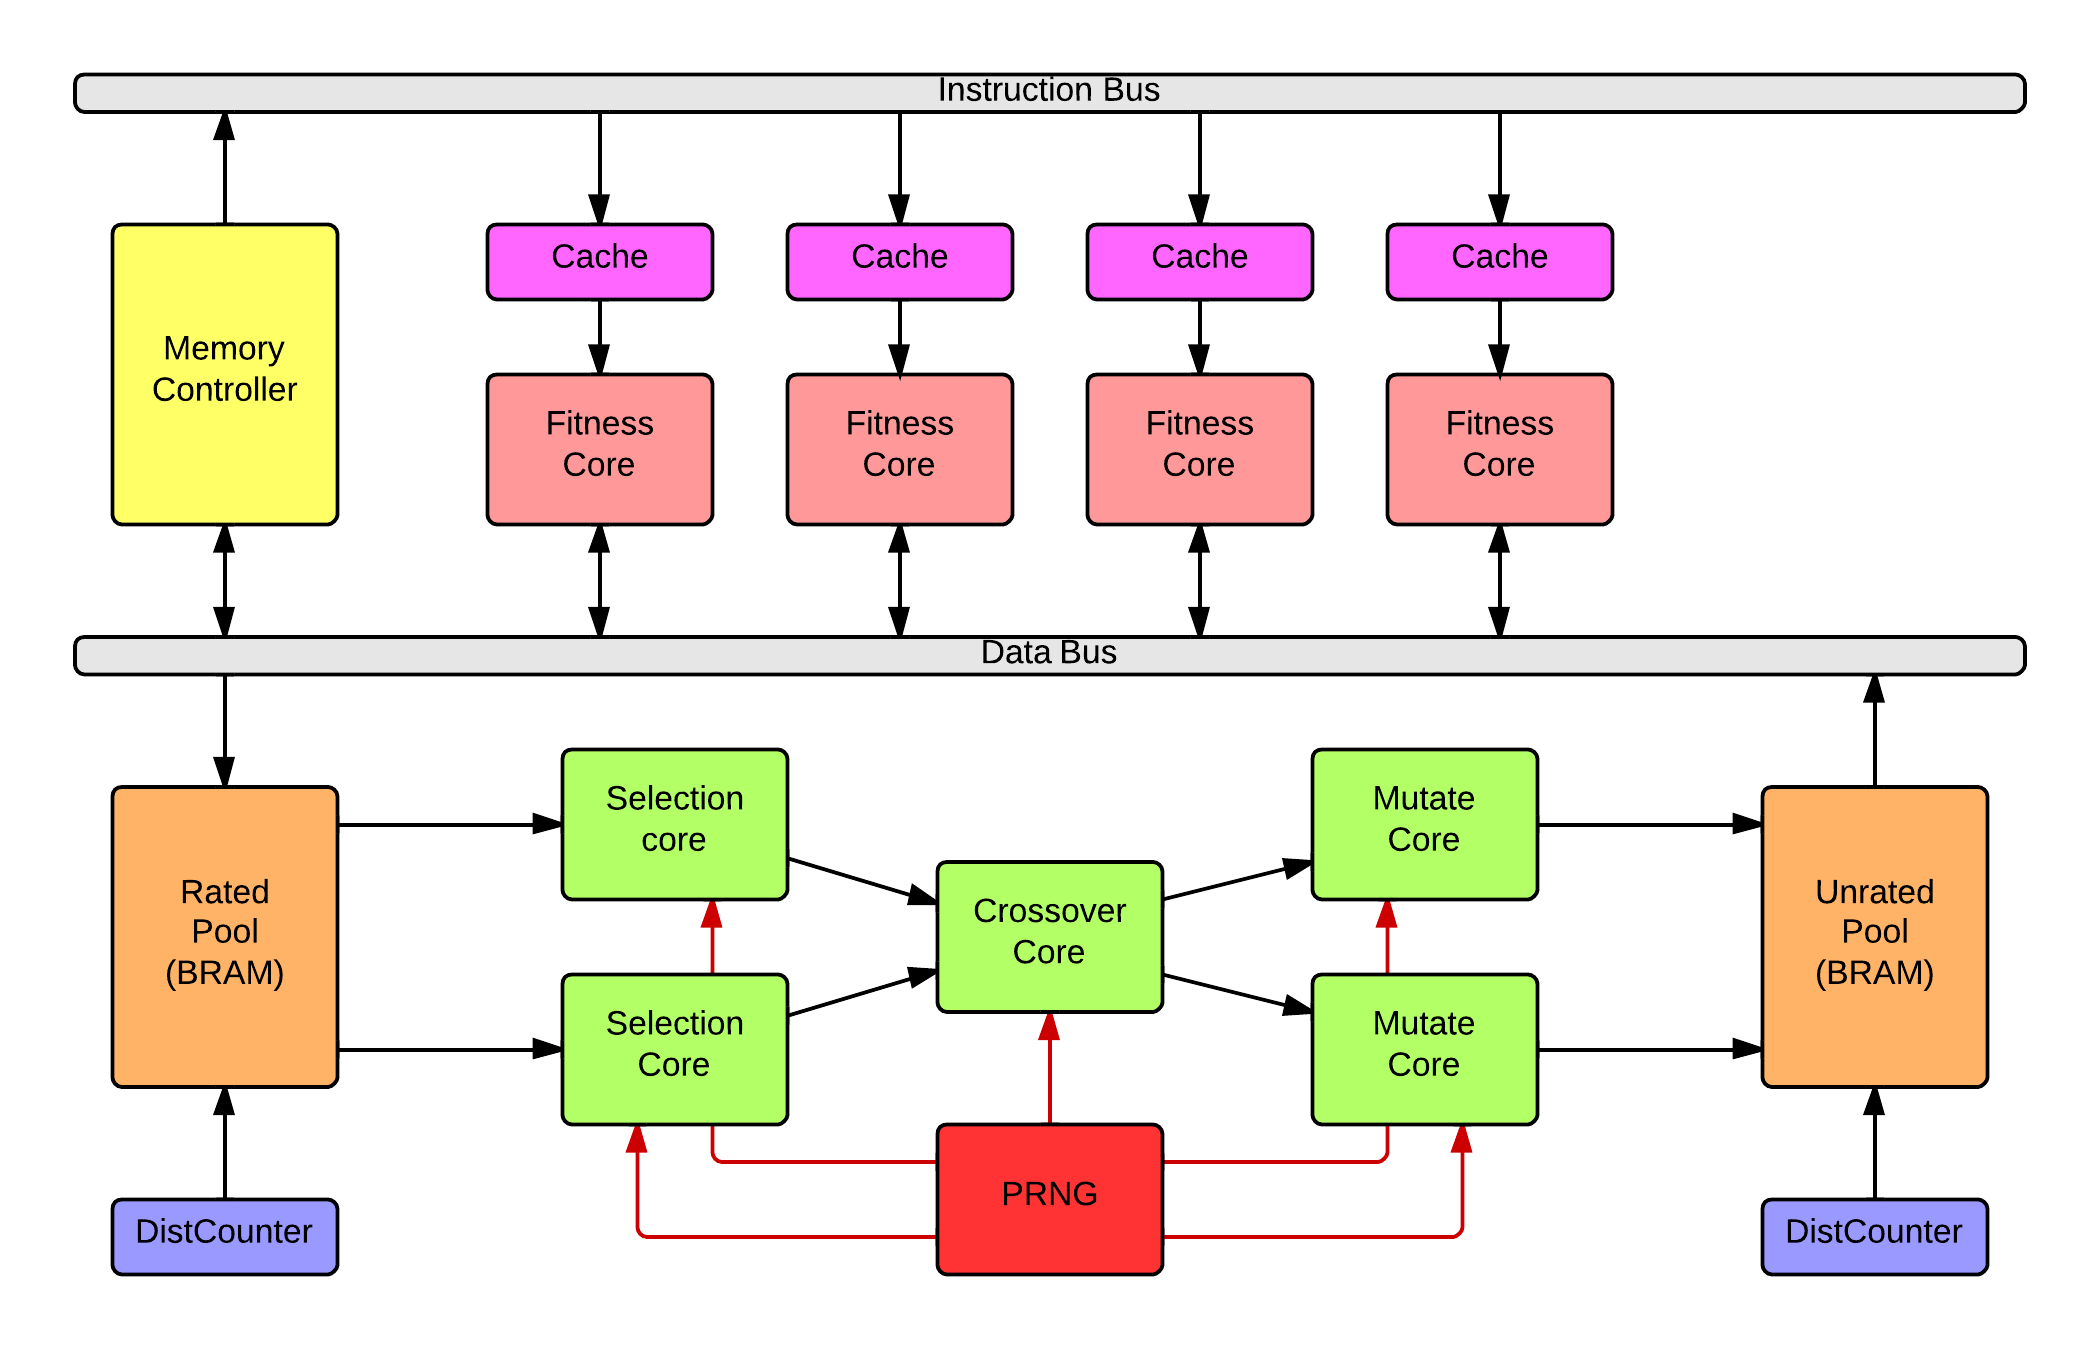
\includegraphics[width=\textwidth]{fpga/fig/processor_architecture.png}
\caption{The figure shows the final processor architecture. Most of the figures seen in this picture as for instance "fitness core", are abstractions of more complex logic at lower levels (mostly MSI and LSI components). }
\label{figure:fpga-architecture}
\end{figure}

\todo{Modify figure \vref{figure:fpga-architecture} so that it is easy to see that the number of fitness cores is configurable.}

The processor architecture designed for the Barricelli computer is a very clean design, and the key to its high performance lies in its simplicity.
The architecture contains a number of general cores, which in this context are named fitness cores.
The fitness cores are general purpose cores in the sense that they are programmable and turing complete, but for genetic algorithm applications the cores are intended to calculate fitness scores of individuals.

The number of fitness cores is configurable.
The reference implementation of the Barricelli computer is configured to have 7 fitness cores.

Common genetic algorithms operations are performed by a separate hardware accelerator pipeline.
This accelerator consists of several operation-specific special cores for selection, crossover and mutation.
The fitness cores and the genetic pipeline are all connected to a single data bus.
To avoid any memory synchronization issues the data bus is controlled by a central arbitration unit.

The processor architecture is illustrated in figure \vref{figure:fpga-architecture}.


\subsection{Instruction Memory}
\label{subsec:fpga-instruction-memory}
The \Gls{barricelli} is a \Gls{harvard machine}.
The memory is split into instruction and data memory.
This is done to achieve better memory throughput, because both memories can be accessed simultaneously.
The instruction memory is organized in a two layer memory hierarchy, with slower external memory (\gls{SRAM}) and faster, internal on-chip caches (\gls{BRAM}).
This separation combines the high instruction thoughput of fast on-board memory wit the comfortably spaceous data storage capabilities of a larger, slower chip external chip.

Each fitness core has its own private instruction memory cache which buffers instructions to decrease the number of slow memory accesses needed during runtime.
Access to an instruction cache is handled by a fitness core's dedicated cache controller, which is responsible for locating and transferring instructions from the instruction memory.
In case of a cache miss, the data-requesting core is halted until the instruction is transferred from memory.
A pseudo-algorithm describing the cache fetch operation can be found in algorithm \vref{algorithm:cache-operation}.
This scheme is created to resolve the conflicts that arise from using shared memory. 

\begin{algorithm}[H]
\SetAlgoLined
\DontPrintSemicolon
\KwData{ $ a = $ an instruction address \newline
$ Ci = $ an array of instructions \newline
$ Ca = $ an array of the corresponding addresses \newline
$ M = $ the instruction memory, indexable by instruction addresses
}
\KwResult{The instruction at address $ a $}
\Begin{
    \If{$ a = Ca[A \bmod{512}] $}{
        \Return{$ Ci[A \bmod{512}] $}
    }\Else{
        $ Caa \bmod{512}] \longleftarrow a $\;
        $ Ci[a \bmod{512}] \longleftarrow M[a] $\;
        \Return{$ Ci[A \bmod{512}] $}
    }
}
\caption{Fetching an instruction from the cache}
\label{algorithm:cache-operation}
\end{algorithm}


\subsection{Data Memory}
\label{subsec:fpga-data-memory}
The \gls{galapagos} architecture is a \gls{MIMD} architecture with shared memory.
In the \Gls{barricelli} computer, a central memory controller is responsible for synchronizing memory access on the shared data bus.
Each component that wants to access memory must go through the memory controller, and follow the proper memory access request protocol.
The controller is constructed in a way that only allows one fitness core to be able to carry out a memory request at a single time.
In case of multiple memory requests, the controller performs a selection deciding in which order the requesting cores is granted the bus.
The precise technique of selection can be seen in algorithm \ref{algorithm:round-robin-selection}.
This may introduce a potential bottleneck for memory-bound problems.
For this reason, each fitness core has a generous 31 general purpose registers, which should reduce the data memory load quite a bit.

\begin{figure}[H]
\begin{algorithm}[H]
\SetAlgoLined
\DontPrintSemicolon
\KwData{$ Requests = $ requests signals from the fitness cores\newline 
$ Request = $ 2-bits specifying the operation}
\Begin{
    $ Requests \longleftarrow $ requests from the fitness cores\;
    \While{$ True $}{
        \For {request in Requests} {
            \If{request $=$ asserted}{
                performMemoryOperation()
            }
        }
        
    }
}
\caption{Round-robin selection}
\label{algorithm:round-robin-selection}
\end{algorithm}
\end{figure}


The selection algorithm is based on round-robin scheduling, and will be explained in further detail here.
The request signals of \emph{fitness cores} are checked in turn to check if one of the cores has requested the memory bus.
The type of request is determined by combination of two request signals sent by each \emph{fitness core}.
The signals refer to either a \emph{NOP}, \emph{READ}, or \emph{WRITE} operation.
In case of \emph{NOP}, the algorithm moves on to check the next state request lines.
It continues doing this in this fashion until a \emph{READ} or \emph{WRITE} request is encountered. 

When a \emph{READ} or \emph{WRITE} operation is encountered, the \emph{data controller} starts to carry out the request from the fitness core.
Performing a memory operation takes at least four cycles, as the processor word size is 64 bits, while the memory bus to the external memory chips are only 16 bits wide.
Because of this, data needs to be shuffled across the bus 16-bits at a time, which accounts for the four cycle minimum for data operations.

For the external memory to be operated correctly by the memory controller, the proper control signals need to be set at the correct times. The signals required differs depending on the type of operation, \emph{READ} or \emph{WRITE}. The timing diagrams can be seen in figure \ref{fpga:fig:timing:dmem:read} and \ref{fpga:fig:timing:dmem:write}, respectively. 

\todo{Check text}

\begin{figure}[H]
  \centering
  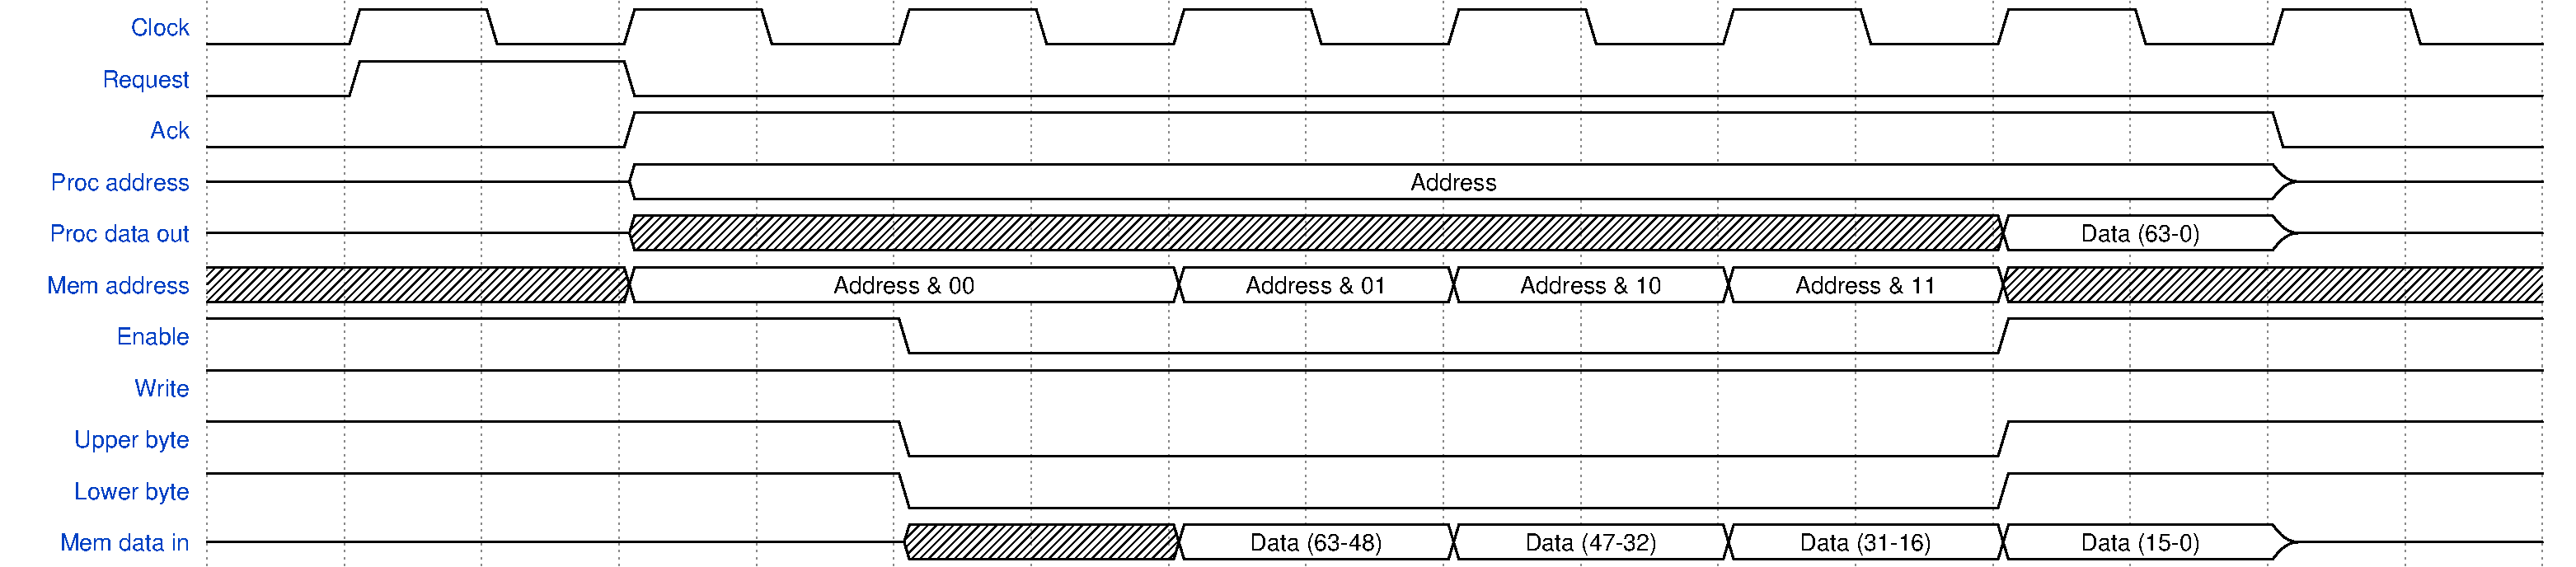
\includegraphics[width=\textwidth]{fpga/fig/timing/data_mem_read.pdf}
  \caption{Data memory read cycle}
  \label{fpga:fig:timing:dmem:read}
\end{figure}

\begin{figure}[H]
  \centering
  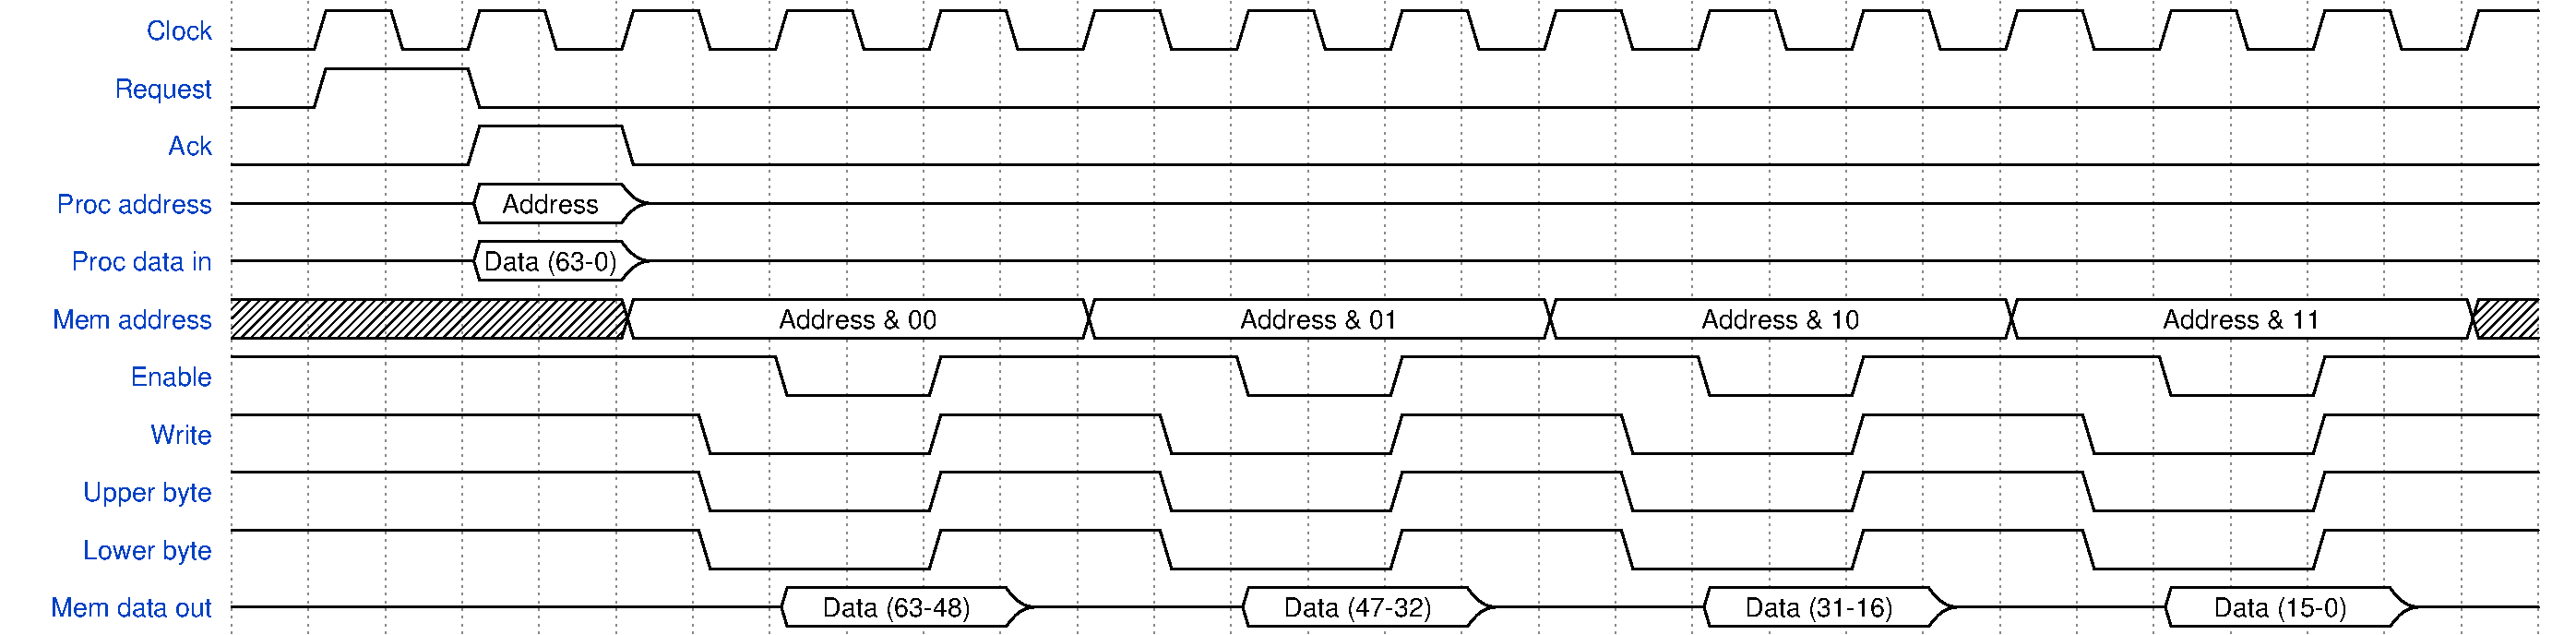
\includegraphics[width=\textwidth]{fpga/fig/timing/data_mem_write.pdf}
  \caption{Data memory write cycle}
  \label{fpga:fig:timing:dmem:write}
\end{figure}

As is immediately apparent in figures \vref{fpga:fig:timing:dmem:read} and \vref{fpga:fig:timing:dmem:write}, the number of cycles required for load and store operations are are 5 and 13 cycles, respectively.
A state machine is implemented in the \emph{data memory controller} to handle interfacing with the external memory chips.
This state machine is responsible for controlling that the different signals are set according to the diagrams.
For more detailed view of the \emph{Data memory controller}, the reader is advised to study the state machine diagram in figure \ref{fpga:fig:mem:data_memory_ctrl_state_machine} and the accompanying data path in figure \ref{fpga:fig:mem:data_memory_ctrl}.

\begin{figure}[H]
  \centering
  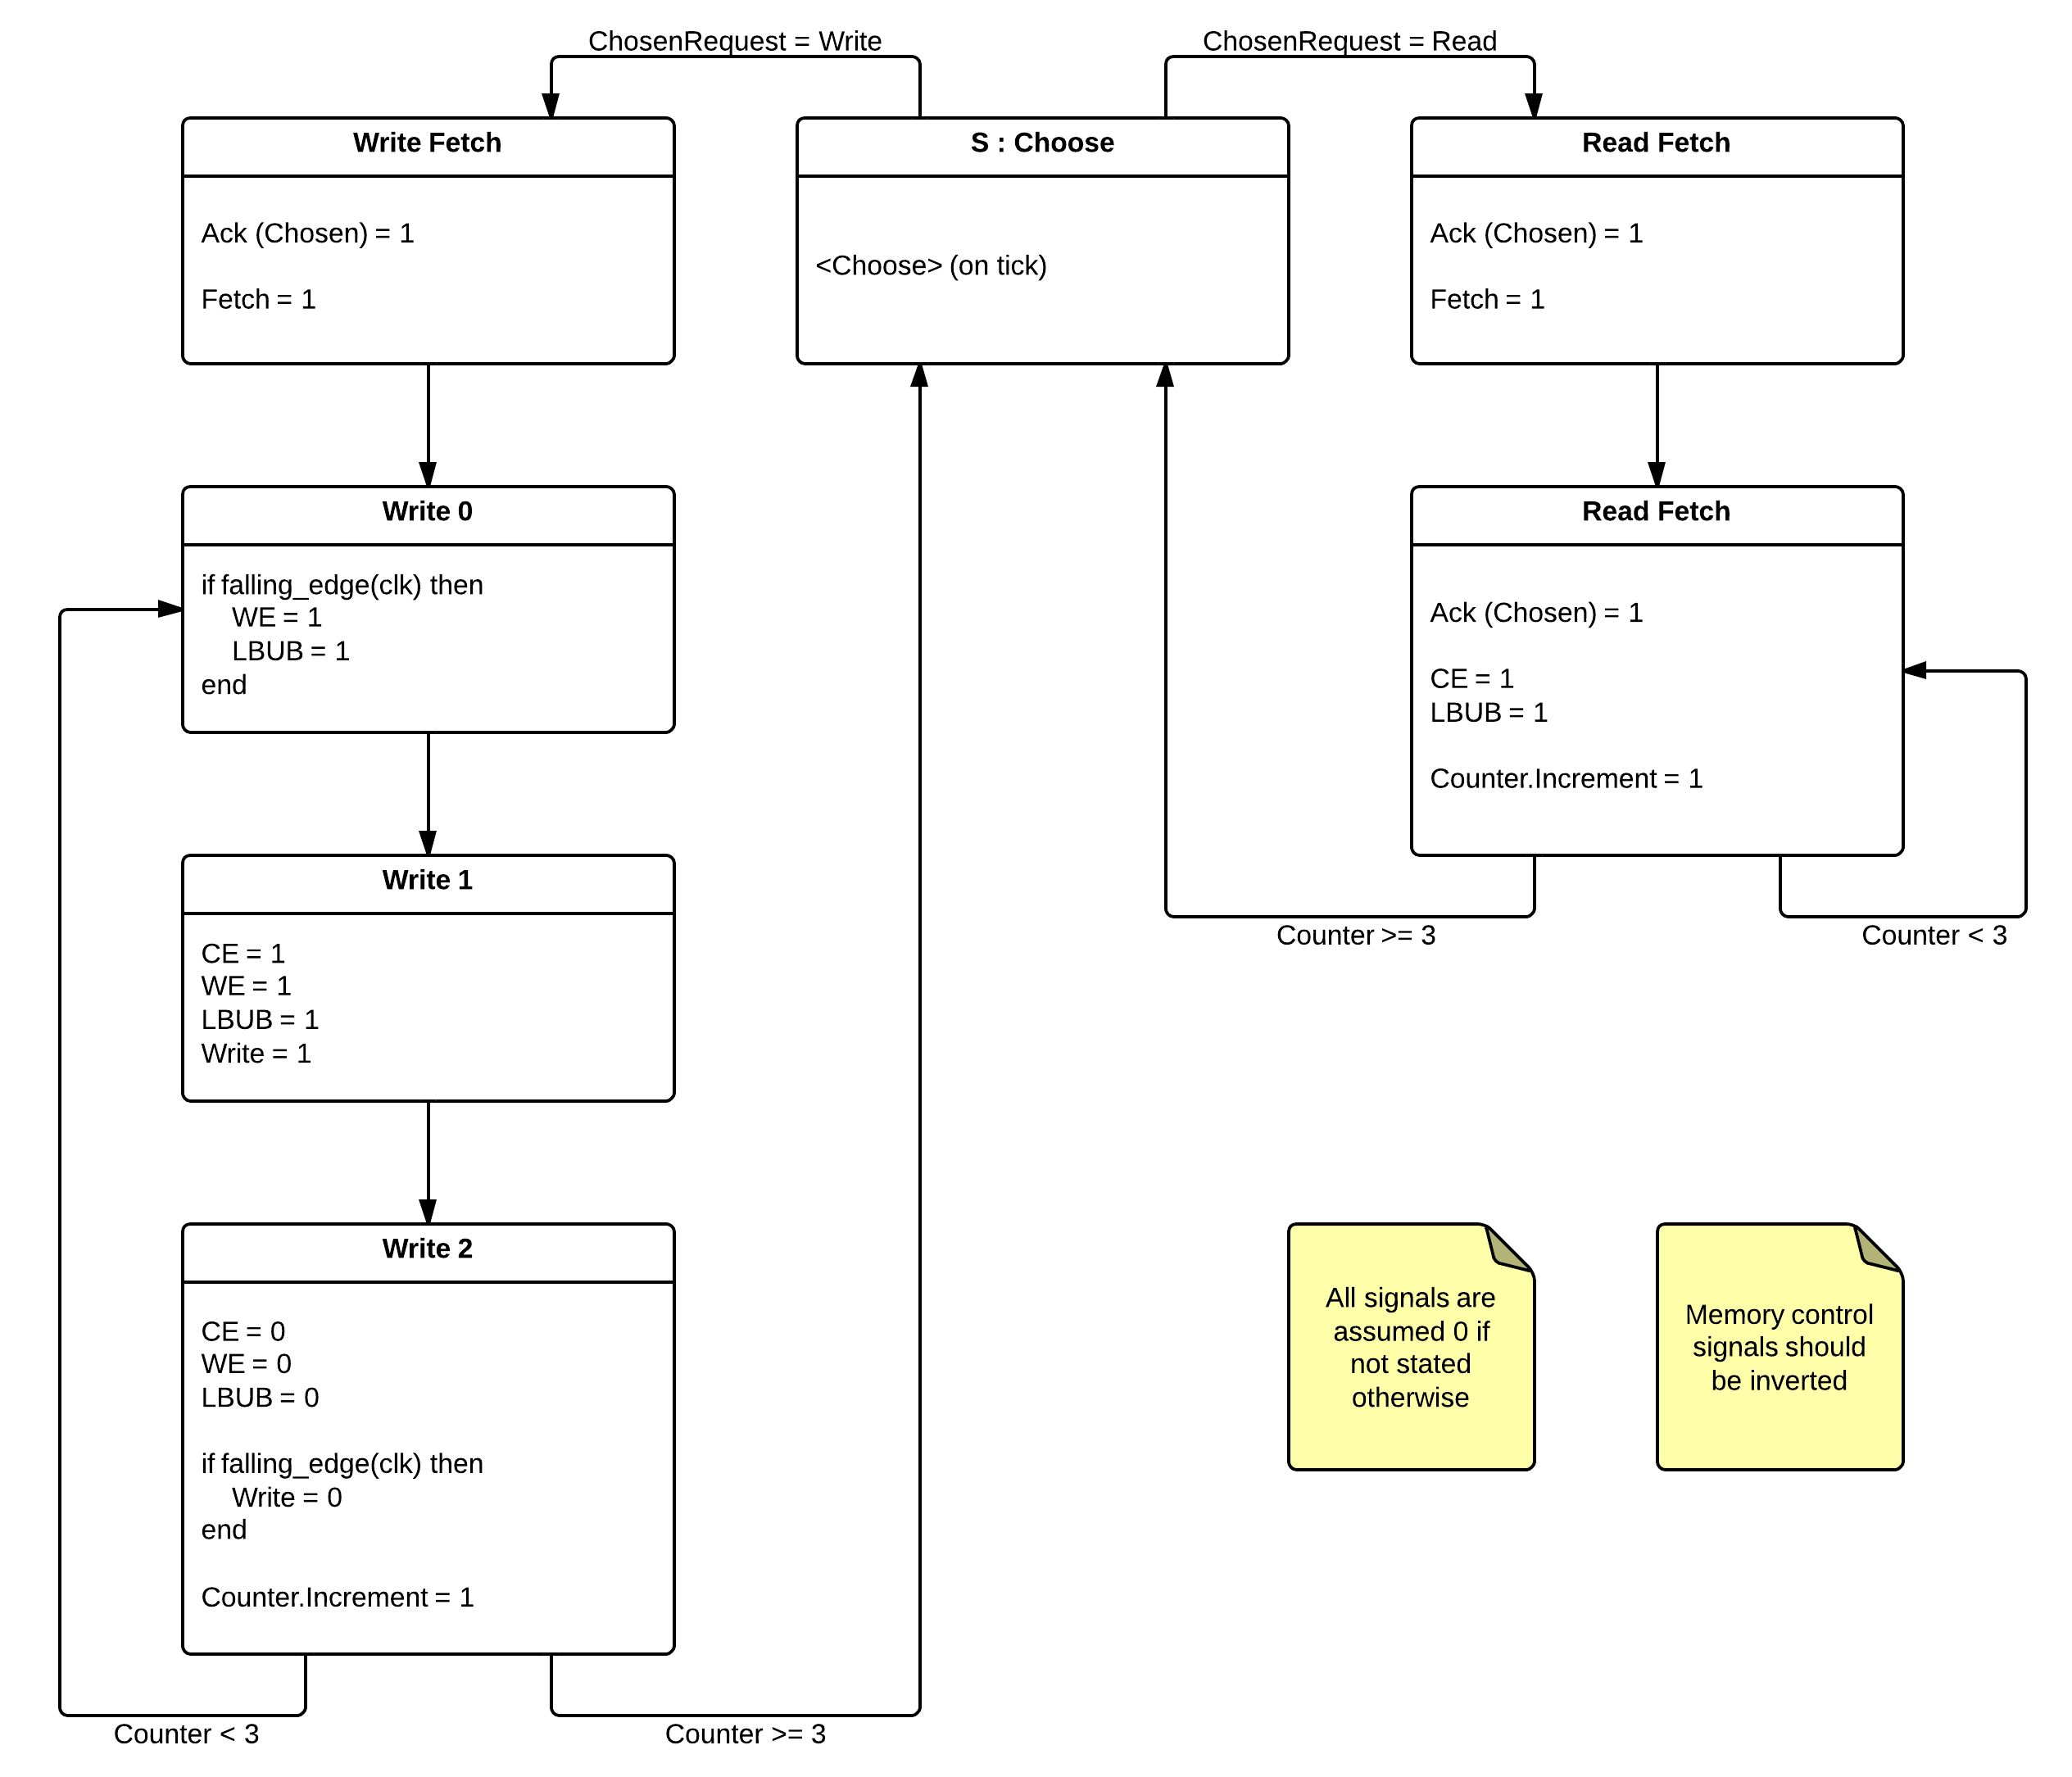
\includegraphics[width=\textwidth]{fpga/fig/memory_ctrl_state_machine.png}
  \caption{Data memory controller state machine}
  \label{fpga:fig:mem:data_memory_ctrl_state_machine}
\end{figure}


\begin{figure}[H]
  \centering
  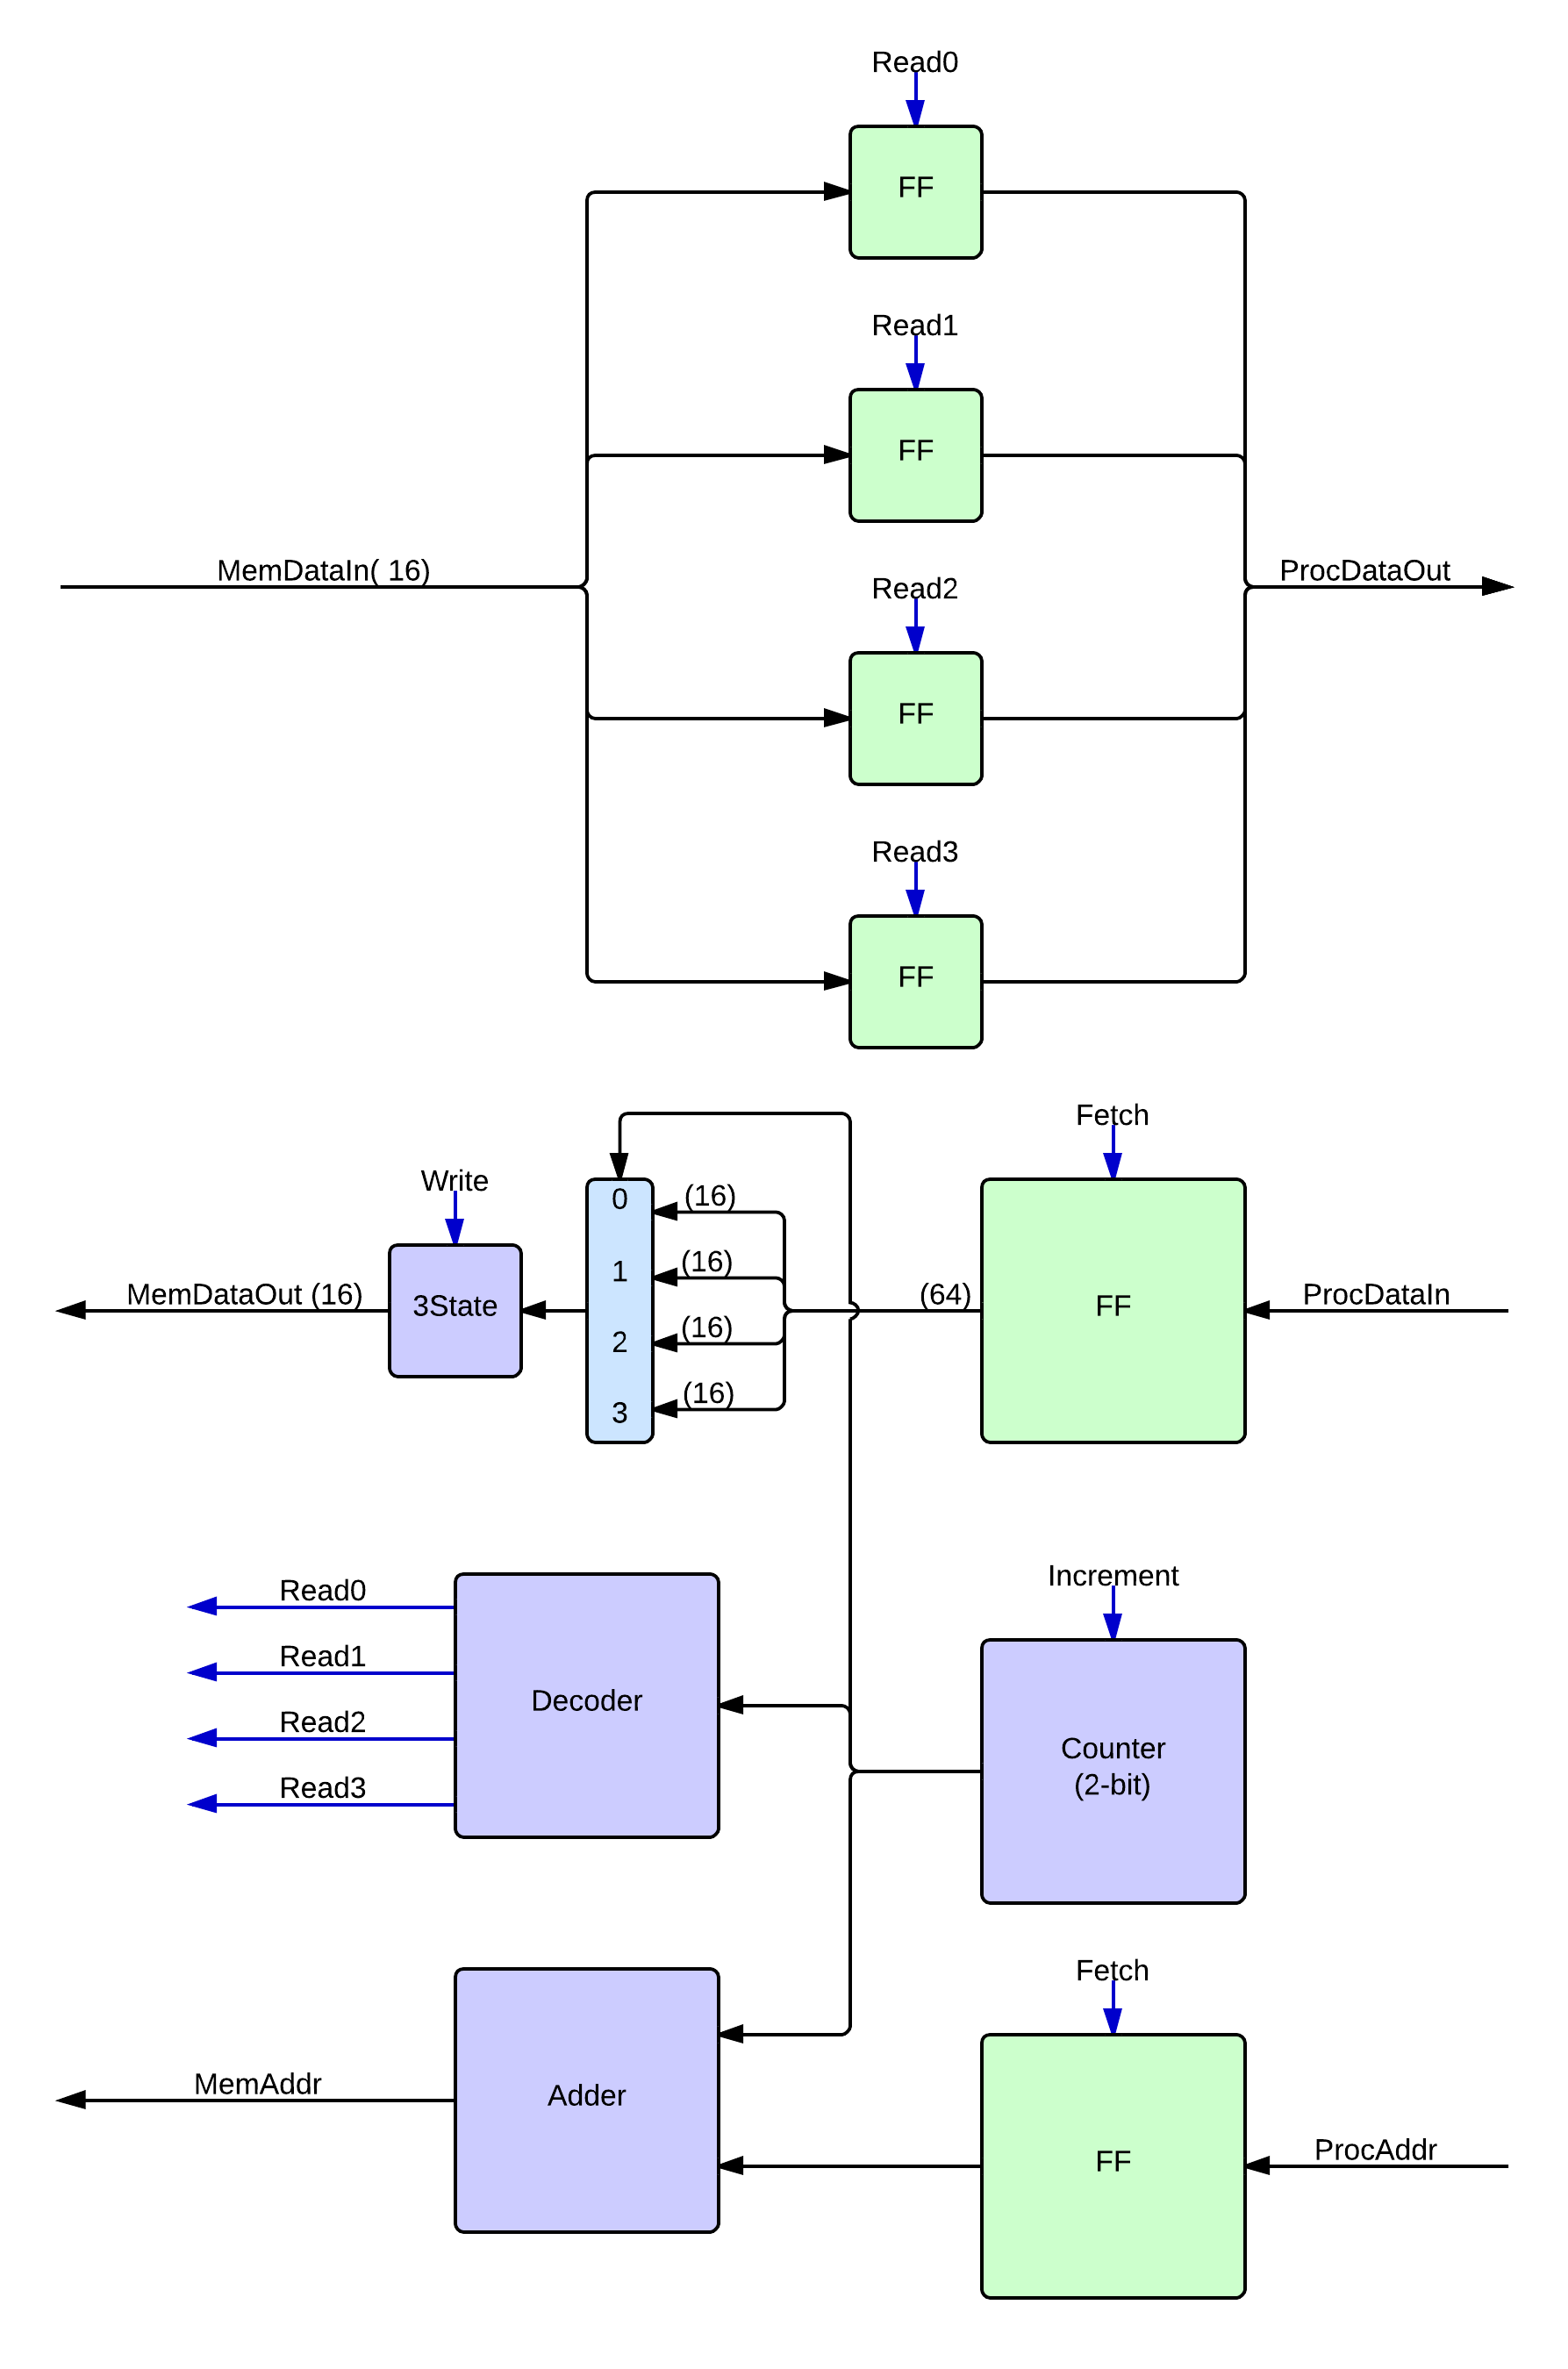
\includegraphics[width=\textwidth]{fpga/fig/memory_ctrl.png}
  \caption{Data memory controller signals mapping}
  \label{fpga:fig:mem:data_memory_ctrl}
\end{figure}


\todo{write about and ref to above graphs}


\subsection{Rated and Unrated Pools}
Individuals making up the populations are stored on the FPGA for for faster access. These are stored in \emph{BRAM} on the FPGA. This implies a lot faster access times, compared to access times to the external memory, as mentioned in (?). This is done to achieve better memory throughput when executing the algorithms. The pools are further divided into two separate \emph{BRAM} blocks, one for rated individuals, and one for un-rated. This is done to achieve even better memory throughput. The increased throughput are achieved because the different computational can work on the rated and un-rated pool simultaneously. For instance while one fitness core is storing a ranked individual, while another fitness core is fetching a new individual for ranking. 

\todo{More details and better explanation} 

Both the rated pool and the unrated pool is associated with the a controller, referred as the \emph{Genetic controller}. As with the data controller, this controller is responsible for granting access for the rated and unrated pool. This buses in question are, however, not the same as those used to access the data memory. The genetic controller use their own separate buses. The controller is based on mostly the same idea as the data controller described in section (?). The when performing genetic operations, the fitness cores need to request the data bus by using two request signals. The combination of these signals refer to the operation the fitness core requests from the genetic controller. 

The genetic cores continuously performs a round-robin in order to grant bus to the requesting fitness core. The logic surrounding the different operations are implemented as an state machine to divide the operations in different clock cycles. This is the same method as used in the data controller.







The state machine can be seen in figure(?)




\subsection{PRNG Module}
The genetic algorithms need diversity in the search space in order to be able to converge to a solution. To achieve this, the architecture need some way of creating sufficiently random numbers. These generated numbers do not need to be true randoms number, this implies that a psudo number generator will suffice. 

    
 

\subsection{Fitness Core} \label{fpga:fitness:ss:design_of_the_fitness_core}
    \subsection{Design of fitness core}

The design of the fitness core is highly influenced by MIPS.
The core is designed as a five stage pipeline.
The goal is to make it as simple as possible, and at the same time harvest efficiency by instruction level parallelism.
The more advanced features like branch prediction and instruction scheduling are not taken into consideration while designing the CPU.
The hazard detection schemes will be made simple.
The hazard resolutions will be made in software as well as in hardware.
The plan is to simply stall when we encounter any hazards in the pipeline.
The assembler will handle the most obvious ones to achieve efficiency, while the hardware will simply stall when hazards are detected.

\fxnote {The hazard scheme may change if time}
 \label{fpga:subsection:fitness_core}


\subsection{The Genetic Pipeline}
\label{fpga:subsection:genetic_pipeline}
\todo{some words about the genetics accelerator}
The galapagos architecture includes a highly specialised pipeline for performing genetic operations. The pipeline is based on the observation that selection, crossover, and mutation works similar for a specific subset of problems. These can therefore be implemented as hardware accelerators constructed for performing one specific task. Constructing such accelerators has been proven to be very beneficial regarding performance. Designing specialised hardware is usually simpler and thereby more effective than constructing general purpose components.\todo{Bullshit ?} This pipeline will effectively relieve the general cores, the fitness cores, from computing the evolution of individuals. The idea is that these will make the fitness cores able to only focus on the computation of fitness ranking, which is considered computational intensive. In the mean time the \emph{genetic pipeline} can produce new data for ranking. These operations could have been performed by the processor, however, the processor is badly suited for these kind of operations. Note that the instructions in the pipeline actually uses 5 cycles in order to complete propagate through the pipeline. It is a far better to only use one cycle in order to complete the one specific operation.  

The genetic pipeline is constructed with three specialised cores for performing selection, crossover, and mutation. These are operations that occurs frequently in genetic algorithms. These are connected to two internal memory banks on the \emph{FPGA}, namely the unrated and rated pool.


-Abstraction for the programmer. Simpler to program.
-Do not need components like ALU
- effective 
- Less control over the genetic pipeline
- 



\subsubsection {Selection Core} \label{fpga:selection:ss:selection_core}
    \input{fpga/selection-core} \label{fpga:subsection:selection_core}

\subsubsection{Crossover Core} \label{fpga:crossover:ss:crossover_core}
    \input{fpga/crossover-core} \label{fpga:subsection:crossover_core}

\subsubsection{Mutation Core}\label{fpga:mutation:ss:mutation_core}
    \input{fpga/mutation-core} \label{fpga:subsection:mutation_core}




\subsection{Parallelism}
\todo{awkwardly placed section.. move it somewhere else?}
The Barricelli is a MIMD computer, which means that it can execute multiple different instruction streams on multiple different data streams simultaneously, in parallel.
The four\cn fitness cores in the archtecture have each their own program counters and may load different data independantly of eachother.
They all share the same data and instruction memory, however, which makes the Barricelli a shared memory model MIMD computer.
Additionally, the genetic pipeline contains multiple specialized cores, which can also execute independant, less general instruction streams on independant data.

 \label{fpga:section:cpu_architecture}


\section{Input/Output}
	\section{Input and Output}
The PCB contains a microcontroller used to manage all input and output between the FPGA and the IO devices shown in Figure ~\vref{figure:system-overview}.
The microcontroller listens on all IO channels for input, and acts on the input, either forwarding the request to another device or performing memory operations on the FPGA's memory.

\subsection{Initial requirements}
The assignment required a microcontroller to handle IO for the FPGA.
To minimize the amount of things that could go wrong, much of the initial work was focused on finding a few reliable and relatively simple data connections.

Specifically, the microcontroller was required to be able to put some program and data on the FPGA's memory, and then later output values from the data memory through the proper communication lines.
The I/O devices together with the microcontroller and it's software should be able to provide a reliable and stable I/O connection between the outside world and the FPGA.

\subsection{Communication channels}
\subsubsection{SD Card}
The SD card reader is primarily used as a storage for programs that are to be uploaded on the FPGA.
However, it might also be used to store memory snapshots in order to look how the genetic algorithm converges to a solution over time.

The Energy Micro Application Note on Fat and SD cards, and its example code, describes an implementation of the FatFS library on the Giant Gecko microcontroller.\cite{an0030}

\paragraph{FatFS}\cite{fatfs-web}

FatFS is a generic FAT file system for microcontrollers, with a generic interface for the FAT operations, and a hardware specific interface for disk I/O.
Because of this structure, the system is easily portable.
To add read and write a FAT system on some disk drive, FatFS needs the following functions:

\begin{table}[H]
    \begin{tabular}{| l | l |}
        \hline
        disk\_initialize & Initialize disk drive \\
        \hline
        disk\_status & Get disk status \\
        \hline
        disk\_read & Read sectors on disk \\
        \hline
        disk\_write & Write sectors on disk \\
        \hline
        disk\_ioctl & Control device dependent features \\
        \hline
        get\_fattime & Get current time for FAT \\
        \hline
    \end{tabular}
    \caption{Overview of disk I/O functions}
\end{table}

\subsubsection{USB}
The USB is the main communication line with a host computer, allowing the host computer to start running programs on the FPGA and receive snapshots of the memory periodically.
The microcontroller has a built in USB controller~\cite{efm32gg990-datasheet} and energy micro has supplied an application note~\cite{an0065} with code for utilizing the included USB controller in order to act as a USB device.

\subsubsection{Serial}
The serial port is meant as a backup solution in case USB doesn't work, with the exact same opportunities, but with an older, simpler interface.
The microcontroller used in the project has a built in UART Receiver/Transmitter\cite{efm32gg990-datasheet} which is easily activated with code from AN0045~\cite{an0045}.

\subsubsection{LEDs and buttons}
The most primitive form of IO we have are the on-board LEDs and buttons.
They allow a quick and easy way to verify that a program is running, and possibly letting the user change execution modes or the program on the FPGA with the buttons.
All code interfacing with the LEDs and buttons are simple code either setting or reading the value of GPIO pins.
The LEDs are driven by General Purpose IO pins on the SCU, requiring a minimal amount of code in order to get a working output, which is especially handy in the early stages of implementation.

\subsubsection{FPGA}
There are 41 wires between the FPGA and the SCU in order to facilitate communication (see Table~\ref{tab:scu-fpga-link} for a complete list of all the connections).
The FPGA has no way of signalling that it wants to output something, so the SCU is responsible for periodically halting the CPU on the FPGA and reading from it's memory.

\subsubsection{J-link}
In order to program and debug the programs on the SCU, we utilize the built-in pins for debugging using J-Link\texttrademark as described in AN0043~\cite{an0043}.
It can also be used as a form of last resort emergency output as it makes it possible to display text that is printed by the program running on the SCU.

\section{FPGA Control}
The only way of communication with the FPGA is with direct memory access to the FPGA's data and instruction memory.
All the data is transferred directly over the SCU's GPIO pins, without any form for memory mapping or built-in bus interfaces.
This is mostly due to the fact that we did not do enough research early in the design process and recognized that we could use something like External Bus Interface to access the memory.

Access to the FPGA's memory is controlled by the signals seen in Table~\ref{tab:scu-fpga-link}.
It should be noted that there are two states to access the FPGA's instruction memory, the upper and lower half.
This is because the instruction memory stores 32 bits per address while the SRAM chips only stores 16 bits per address (see Section~\ref{subsec:fpga-instruction-memory} for more details on the instruction memory).

The SRAM data sheet~\cite{sram-datasheet} specifies that the data signal has to be stable for at least 10ns in order to complete a write.
This means that it is not necessary to worry about timing when accessing the SRAM since changing the signal more than every 10ns requires a clock speed of 100MHz since we can at most change the output of a single pin every cycle.

\begin{table}[H]
    \begin{tabular}{| l | l | l |}
        \hline
        Signal & Bus width & \\
        \hline
        FPGA enable & 1 & Enables the FPGA on high, disables it on low\\
        \hline
        FPGA State & 2 & \pbox{20cm}{00: Processor enable\\01: Instruction memory upper half access\\10: Instruction memory lower half access\\11: Data memory access}\\
        \hline
        Chip enable & 1 & The chip enable signal in to the selected memory block.\\
        \hline
        Write enable & 1 & The write enable signal in to the selected memory block.\\
        \hline
        Address & 19 & The address bus to the selected memory block.\\
        \hline
        Data & 16 & The data bus to the selected memory block.\\
        \hline
        LBUB & 1 & The LB and the UB signal to the selected memory block.\\
        \hline
    \end{tabular}
    \label{tab:scu-fpga-link}
    \caption{Lines between the SCU and FPGA}
\end{table}

\section{IO Program}
\begin{figure}[H]
    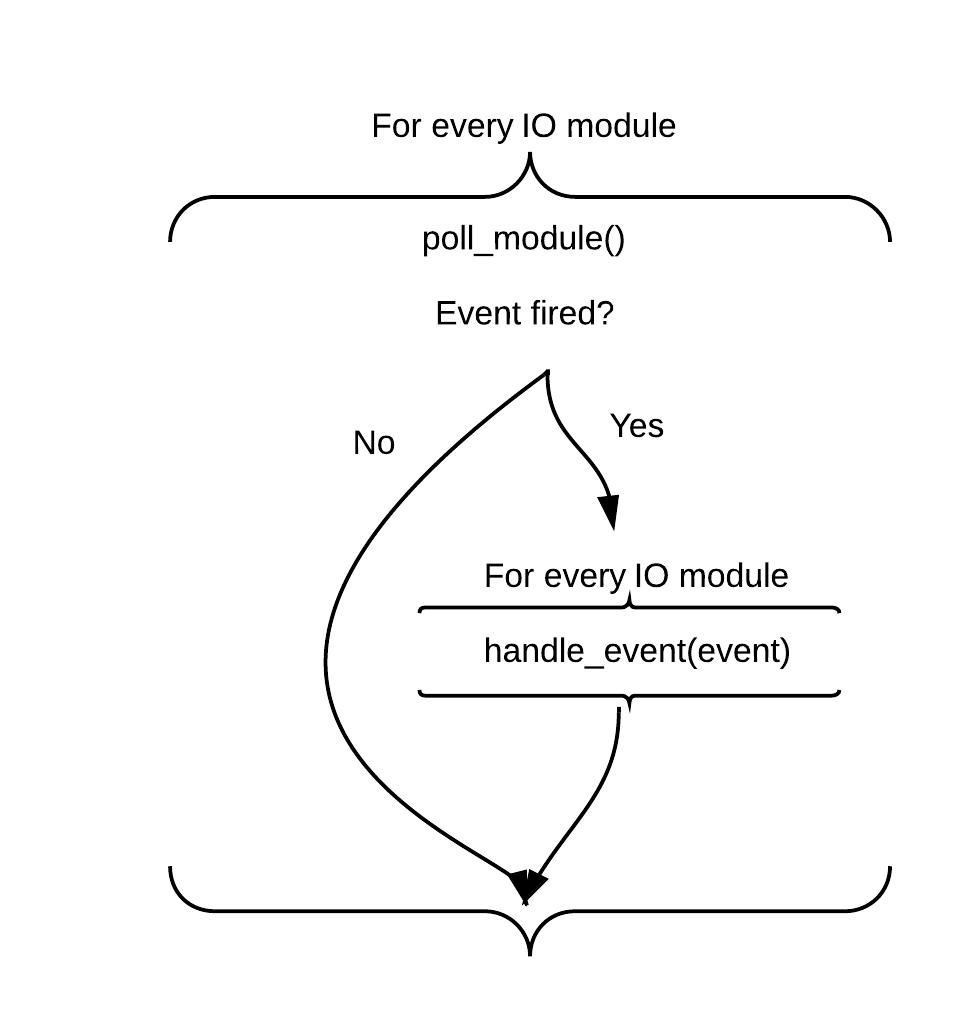
\includegraphics[width=\textwidth]{io/fig/program.png}
    \caption{The body of the IO program's main loop}
\end{figure}

The IO program was designed to be as simple as possible in order to decrease the amount of things that could go wrong.
The main idea is that every IO device is required to define two functions in order to be used: a function to poll for input and a function that is called whenever a device reports input.

In order to enable sending messages between different IO units, the poll functions return a pointer which may point to any object in memory, which allows other modules to read the data given that they know what type of data the pointer points to.

\section{Design decision}
\subsection{Selection of microcontroller}
The microcontroller chosen was chosen as it was the microcontroller we had available to test with on the development kit.
It was also the microcontroller with most available GPIO pins for the package we had to use, which would give us the most possibilities for communication.

\subsection{Operating system}
Early in the process, a discussion arose about how it could be beneficial to run an operating system on the microcontroller such that familiar programs could be run directly on it.
A scenario pitched was to have network access, and then be able to talk to the machine remotely using programs such as \textit{SSH} or \textit{telnet}.
However, the Linux distribution available for the Energy Micro microcontroller was found lacking in the features we wanted, and the microcontroller lacks network support.
It was therefore decided that running an OS was unnecessary as there were few rewards and little to gain from it.

\subsection{FPGA Communication}
During the initial design phase, the link between the FPGA and SCU was designed to be as simple as possible.
The final version was the the 41 wires mapping all the signals needed for directly accessing the SRAM chips.
\todo{Make up some reasons here, should probably defend not using EBI}

\section{Issues}
\subsection{Crystal}
In the design phase it was decided to go with just a single high frequency crystal oscillator.
Unfortunately the crystal that was selected had a clock frequency in the kHz range, instead of the MHz range, which was what was intended.
Luckily the microcontroller has a built-in RC oscillator, so the crystal oscillator was not essential to get code running on the microcontroller.

\subsection{USB Circuitry not working}
While mapping the PCB circuitry, only the pins available for GPIO were included initially, but this did not include the vbus and vregi pins.
The pins were connected to capacitors, and a quick hack soldering the appropriate lines to the USB header was tried without success.

\subsection{No UART}
The microcontroller believes that data is being outputted and calls the data sent callback function.
There also seems to be a signal going out to the RS-232 interface, but there is no data being received on the other end.

\todo{no SD card}

\subsection{Memory access}
\todo{Diagnostics, possibly not just here/not here at all.}
Tried:
\begin{itemize}
    \item Adding delays
    \item Reading immediately after write to verify write,
    \item Mapping control signals to LED on FPGA to verify that they work
    \item Flashing the instruction memory on the FPGA so we just have to read data memory, not write
\end{itemize}


\section{Conclusion}

\part{Test report}

\section{Testing}
	When designing a computer with a custom architecture from scratch, it is important to continually test and evaluate the correctness of the solution at all possible stages, to ensure that final product is a success.
This section documents and explaines the rationale behind the different types of tests that have been performed.

\section{Testing the Processor}

Baricelli's processor has been tested at four different levels: \gls{VHDL}-based unit test simulations of the different subcomponents,  \gls{VHDL}-based integration test simulations of each processing unit, \gls{VHDL}-based system test simulations of the entire system interfacing against a mock SCU and mock memory, and finally physical integration tests of the processor programmed onto the FPGA of the Barricelli.

\todo{what about timing simulations?}

\subsection{\gls{VHDL}-based Subcomponent Unit Test Simulations}

Unit testing VHDL entites is extremely important in a large and complex design like the Barricelli.
For this project, almost every component, perhaps except the most trivial entities, is tested in an automated or semi-automated VHDL test bench.
A tool was developed to ease the automation of VHDL test running and validation, modeled after the leading test runners in the software industry, such as JUnit\cn and Karma\cn.
This tool enabled tests to be written using easy-to-use self-evaluating tests that compare signals at specific times against expected values.

The goal of these unit tests is to ensure that the building block components work as expected when reacting to specified input.

Screenshots of simulations of these tests can be found in Appendix \ref{appendix:test-bench-documentation}.
\todo{ Make sure screenshots of as many tests as possible are available. If not, then we probably have to do references from the following tables}
\todo{we need to stash results somewhere}.

\subsubsection{Fitness Core Components}
\todo{ Insert text and tables for components used in Fitness Core}

\subsubsection{Genetic Pipepline Components}
\todo{ Insert text and tables for components used in Genetics Pipeline}
\paragraph{Selection Core}
\paragraph{Genetic Pipeline Controller?}
\paragraph{Unrated pool?}
\paragraph{Rated pool?}

\todo{ Hmm...seems I overdid the length in the tables. Again!....(T-Bear)}
\begin{table}[H]
  \begin{tabular}{r | p{9cm}}
    \noalign{\smallskip}\hline\noalign{\smallskip}
    
    What to test:  & Check if crossover split function performs crossover correctly, 
                        from correct bit \\

    \noalign{\smallskip}\hline\noalign{\smallskip}

    How to test:   &    Changes in any input should cause change in the outputs.
                        Therefore parent inputs and random\_number will be changed
                        during test. 
                        \\
                      
    \noalign{\smallskip}\hline\noalign{\smallskip}

    Pass criteria: &    The output for child1 should have output from parent1 and child2
                        from parent2 before crossover point, and child1 should have
                        output from parent2 and child2 from parent1 after crossover
                        point. 
                        The starting point, which is the first bit in the crossover,
                        should always be the bit number equal to the value of
                        random\_number.
                        \\
    \noalign{\smallskip}\hline\noalign{\smallskip}
    
    Results: &      Successful. 
                    Changes in parents cause expected changes in children, and starting 
                    point for crossover is always equal to the value of random\_number
                    \\
   \noalign{\smallskip}\hline\noalign{\smallskip}
  
  
  
  \end{tabular}
  \caption{Crossover Core Split function}
  \label{testing:components:genetic_pipeline:crossover_core_split}
\end{table}

\begin{table}[H]
  \begin{tabular}{r | p{9cm}}
    \noalign{\smallskip}\hline\noalign{\smallskip}
    
    What to test:  & Check if Crossover Double-Split Function performs crossover
                     correctly, from correct starting bit to correct ending bit \\

    \noalign{\smallskip}\hline\noalign{\smallskip}

    How to test:   &    Changes in any input should cause change in the outputs.
                        Therefore parent inputs and random\_numbers will be changed
                        during test.  
                        \\
                      
    \noalign{\smallskip}\hline\noalign{\smallskip}

    Pass criteria: &    The output for child1 should have output from parent1 and child2
                        from parent2 before crossover starting point and after ending 
                        point, and child1 should have output from parent2 and child2
                        from parent1 between the crossover starting point and ending
                        point. 
                        The random\_number with the highest value should always be the 
                        starting point, and the one with the lowest value should always
                        be the ending point. 
                        These points, which are the first and the last bit in the 
                        crossover, should always be the bit numbers equal to the value     
                        of the random\_numbers. 
                        If both have same value, then only one bit location will have a
                        crossover
                        \\
    \noalign{\smallskip}\hline\noalign{\smallskip}
    
    Results: &      Successful. 
                    Changes in parents cause expected changes in children, and starting 
                    point for crossover is always equal to the value of the highest 
                    random\_number, and ending point for crossover is always equal to 
                    the value of the lowest random\_number
                    \\
   \noalign{\smallskip}\hline\noalign{\smallskip}
  
  
  
  \end{tabular}
  \caption{Crossover Core Double-Split function}
  \label{testing:components:genetic_pipeline:crossover_core_doublesplit}
\end{table}

\begin{table}[H]
  \begin{tabular}{r | p{9cm}}
    \noalign{\smallskip}\hline\noalign{\smallskip}
    
    What to test:  & Check if Crossover XOR Function performs crossover
                     correctly, from correct starting bit to correct ending bit \\

    \noalign{\smallskip}\hline\noalign{\smallskip}

    How to test:   &    Changes in any input should cause change in the outputs.
                        Therefore parent inputs and random\_number will be changed
                        during test.  
                        \\
                      
    \noalign{\smallskip}\hline\noalign{\smallskip}

    Pass criteria: &    The output for child1 should have output from parent1 and child2
                        from parent2 for each bit \emph{i}, where in the random\_number 
                        the value is 0, and child1 should have output from parent2 and 
                        child2 from parent1 for each bit \emph{i}, where in the 
                        random\_number the value is 1.
                        \\
    \noalign{\smallskip}\hline\noalign{\smallskip}
    
    Results: &      Successfull.
                    Changes in parents cause expected changes in children, and for each
                    bit \emph{i} in the random\_number, there are crossover at same bit    
                    \emph{i} from the parents to the children.
                    \\
   \noalign{\smallskip}\hline\noalign{\smallskip}
  
  
  
  \end{tabular}
  \caption{Crossover Core XOR function}
  \label{testing:components:genetic_pipeline:crossover_core_xor}
\end{table}

\begin{table}[H]
  \begin{tabular}{r | p{8cm}}
    \noalign{\smallskip}\hline\noalign{\smallskip}
    
    What to test:  & Check if Crossover Toplevel selects correct crossover function
                     based on control\_input, and random\_number when in "Party Mode"\\

    \noalign{\smallskip}\hline\noalign{\smallskip}

    How to test:   &    Changes in parents are not relevant, since this test is not 
                        inteded to test the functions themselves, only the function 
                        selection.
                        Every input of control\_input will be tested.
                        Changes in random\_number will be done with focus on the 2 LS 
                        bits when control\_input is "1XX", and in party mode.
                        \\
                      
    \noalign{\smallskip}\hline\noalign{\smallskip}

    Pass criteria: &    When control\_input is set to 000, or 1XX and random\_input-bits 
                        to 00, crossover should be split with the value of the 6 LS bits 
                        from random\_number used for starting point.
                        When control\_input is set to 001, or 1XX and random\_input-bits 
                        to 01, crossover should be double-split, with the value of the 
                        12 LS bits from random\_number used for starting and ending 
                        point.
                        When control\_input is set to 010, or 1XX and random\_input-bits 
                        to 10, crossover should be xor, with crossover on every bit 
                        numbers that are 1 in random\_number.
                        When control\_input is set to 011, or 1XX and random\_input-bits 
                        to 11 there should be no crossover at all, and output children 
                        should be equal to each their input parent.
                        \\
    \noalign{\smallskip}\hline\noalign{\smallskip}
    
    Results: &      Successfull. 
                    Each value in control\_input was tested, and set the expected 
                    function. When set to 1XX, every value on the 2 LS bits in the 
                    random\_number was tested, and set the expected function.
                    \\
   \noalign{\smallskip}\hline\noalign{\smallskip}
  
  
  
  \end{tabular}
  \caption{Crossover Core Toplevel}
  \label{testing:components:genetic_pipeline:crossover_core_toplevel}
\end{table}

\begin{table}[H]
  \begin{tabular}{r | p{9cm}}
    \noalign{\smallskip}\hline\noalign{\smallskip}
    
    What to test:  & Check if Mutation Core selects mutates when allowed, mutates the 
                     correct amount of bits, and the correct bit numbers, all based
                     on chance\_input and random\_number.\\

    \noalign{\smallskip}\hline\noalign{\smallskip}

    How to test:   &    Changes on input will change output. Therefore input will have 
                        changes.
                        Changes in random\_number and chance\_input  will be done with
                        focus to test allowing or denying mutation.
                        Changes in random\_number will also be done to test amount of 
                        allowed mutations, and to test selecting the locations of the 
                        mutations
                        \\
                      
    \noalign{\smallskip}\hline\noalign{\smallskip}

    Pass criteria: &    When the P first bits in random\_number is equal to or higher 
                        than chance\_input (size P), there should be no mutation at all.
                        When mutation is allowed, the next two bits should allow these 
                        amount of mutations: 1-4 depending on values 00-11.
                        Bits 23-0 select four bit locations for mutations, and the 
                        output should have opposite value on these locations compared to
                        the input.
                        If more than one bit location pointer has the same value, the 
                        same bit location should still have the mutation on the output.
                                                \\
    \noalign{\smallskip}\hline\noalign{\smallskip}
    
    Results: &      Successful. 
                    Mutation is allowed only when the P first bits are lower than the
                    chance\_input, the correct amount of mutations were set and each 
                    four bit locations were selected correctly as expected by bits 23-0
                    \\
   \noalign{\smallskip}\hline\noalign{\smallskip}
  
  
  \end{tabular}
  \caption{Mutation Core}
  \label{testing:components:genetic_pipeline:mutation_core}
\end{table}



\subsubsection{Components stolen from AREA 51}
\todo{ Insert text and tables for components used elsewhere}

\subsection{\gls{VHDL}-based Processing Unit Integration Test Simulations}

Each processing unit, which each consists of several interconnected subcomponents, has been simulated for integration testing.
The goal of these tests are to verify that the different subcomponents interface correctly with eachother, and that the behaviour of the supercomponent is as expected.

\subsubsection{Testing the Fitness Core}

\todo{about tb\_fitness\_core.vhd}

\subsubsection{Testing the Genetics Pipeline}

\todo{about tb\_genetics\_pipeline.vhd}

\subsection{\gls{VHDL}-based System test Simulations}
\label{section:testing:fpga:system-tests}

The toplevel simulation test bench of the barricelli computer, which simulates the entire FPGA as a black box interfacing against the external components, supports pre-loading entire programs into a mocked instruction memory component.
The \Gls{galapagos assembler} supports outputting assembled programs compiled to one of these mock memory components, meaning that testing new programs in a simulated environment is an easy and fun process.

\todo{the title of the test should be above the table in which its results are displayed, not just as the caption (rendered below) of the table}

A formal description of the system tests performed at this level can be found in tables
\ref{testing:fitness:pipeline_test},
\ref{testing:fitness:branch_taken},
\ref{testing:fitness:branch_not_taken},
\ref{testing:fitness:conditional_taken},
\ref{testing:fitness:conditional_not_taken},
\ref{testing:fitness:load_data},
\ref{testing:fitness:store_data},
\ref{testing:fitness:store_gene},
and
\ref{testing:fitness:load_gene}.

\begin{table}[H]
  \begin{tabular}{r | p{8cm}}
    \noalign{\smallskip}\hline\noalign{\smallskip}
    
    What to test:  & Observe that RRI and RRR instructions propagate correctly through the pipeline, 
                     and produce the correct result.\\

    \noalign{\smallskip}\hline\noalign{\smallskip}

    How to test:  & The program in listing \todo{create listing}, consisting of both RRR and RRI instructions,
                    are loaded into memory with the test framework. The execution of the instructions are observed with
                    isim.\\

    \noalign{\smallskip}\hline\noalign{\smallskip}

    Pass criteria: & The flow of data is according to the architecture presented in figure. \todo{add reference}
                   Register 1, 2, 3 are loaded with 9, 10 and 19, respectively.   \\
    
     \noalign{\smallskip}\hline\noalign{\smallskip}

    Results: &  What are the result of the test. \\
   \noalign{\smallskip}\hline\noalign{\smallskip}
  
  
  \end{tabular}
  \caption{RRR and RRI instructions}
  \label{testing:fitness:pipeline_test}
\end{table}


\begin{table}[H]
  \begin{tabular}{r | p{8cm}}
    \noalign{\smallskip}\hline\noalign{\smallskip}
    
    What to test:  & Check if the branch address is calculated correctly, and an conditional
                     jump is performed to this address. \\

    \noalign{\smallskip}\hline\noalign{\smallskip}

    How to test:   &  The program in listing \todo{create listing}, is loaded into a test bench.
                      This simple program consists of a simple loop performing some arithmetic
                      operations that store values to registers. The execution of the
                      program is simulated with isim to verify the result \\

    \noalign{\smallskip}\hline\noalign{\smallskip}

    Pass criteria: &  The branch is taken. The instructions located in the $fetch stage$, 
                       $decode stage$, and $execute stage$ are flushed. The results in registers
                       should be X, X, and X in registers X, X and X, respectively. \\

    \noalign{\smallskip}\hline\noalign{\smallskip}
    
    Results: &  Registers X, X, and X is contained in the registers. The instructions in $fetch
                stage$, $decode stage$ and $execute stage$ does not perform any  
                changes to the register file. \\
   \noalign{\smallskip}\hline\noalign{\smallskip}
  
  
  
  \end{tabular}
  \caption{Branch taken}
  \label{testing:fitness:branch_taken}
\end{table}

\begin{table}[H]
  \begin{tabular}{r | p{8cm}}
    \noalign{\smallskip}\hline\noalign{\smallskip}
    
    What to test:  & Check if the conditional jump is disregarded when performing conditional
                     that always evaluate to false.\\

    \noalign{\smallskip}\hline\noalign{\smallskip}

    How to test:   &  The program in listing \todo{create listing}, is loaded into a test bench. 
                       The simple program consists of conditionals that evaluate to false. The
                       execution of the program is simulated with isim, and the results are
                       verified. \\

    \noalign{\smallskip}\hline\noalign{\smallskip}

    Pass criteria: & Execution of the program should not store any data to the registers.\\

    \noalign{\smallskip}\hline\noalign{\smallskip}
    
    Results: &   No data is stored to registers. \\
   \noalign{\smallskip}\hline\noalign{\smallskip}
  
  
  
  \end{tabular}
  \caption{Branch not taken}
  \label{testing:fitness:branch_not_taken}
\end{table}

\begin{table}[H]
  \begin{tabular}{r | p{8cm}}
    \noalign{\smallskip}\hline\noalign{\smallskip}
    
    What to test:  & Check if conditional instruction are executed when they
                     always are evaluated to true.   \\

    \noalign{\smallskip}\hline\noalign{\smallskip}

    How to test:  & The program in listing \todo{create listing}, is loaded into test bench. The 
                    simple program consists of a set with simple conditional instructions that
                    always evaluate to true. The execution of the program is simulated with isim, 
                    and the result is verified. 
    \\

    \noalign{\smallskip}\hline\noalign{\smallskip}

    Pass criteria: & The instructions propagates normally through the pipeline. The different instruction are executed and their results are written to the register file. \\

    \noalign{\smallskip}\hline\noalign{\smallskip}
    
    Results: &  \\
   \noalign{\smallskip}\hline\noalign{\smallskip}
  
  
  
  \end{tabular}
  \caption{Conditional instruction executed }
  \label{testing:fitness:conditional_taken}
\end{table}

\begin{table}[H]
  \begin{tabular}{r | p{8cm}}
    \noalign{\smallskip}\hline\noalign{\smallskip}
    
    What to test:  & Check if conditional instructions are executed when they always evaluate to 
                     false. \\

    \noalign{\smallskip}\hline\noalign{\smallskip}

    How to test:   &  The program in listing \ref{testing:listing:conditional-not_executed}, is loaded into a test bench. 
                       The simple program consists of a set of simple conditional instructions that         
                       always evaluate to false. The execution of the program is observed in 
                       ISim,and the results are verified. The content of register r1 is observed.\\

    \noalign{\smallskip}\hline\noalign{\smallskip}

    Pass criteria: & The second instruction, the conditional \emph{ADDI}, is not executed. The content of register r1 is 1.  \\

    \noalign{\smallskip}\hline\noalign{\smallskip}
    
    Results: & The content of register r1 is 1. The conditional \emph{ADDI} instruction is not executed. .  \\
   \noalign{\smallskip}\hline\noalign{\smallskip}
  
  
  
  \end{tabular}
  \caption{Conditional instruction not executed}
  \label{testing:fitness:conditional_not_taken}
\end{table}

\begin{table}[H]
  \begin{tabular}{r | p{8cm}}
    \noalign{\smallskip}\hline\noalign{\smallskip}
    
    What to test:  & Observe that LOAD instructions is able to read from memory, and load the
                     memory content into the specified registers.  \\

    \noalign{\smallskip}\hline\noalign{\smallskip}

    How to test:   & The program in listing \todo{create listing}, consisting mainly of LOAD
                     instructions. These are loaded into a testbench, and simulated with 
                     isim. \\
                     

    \noalign{\smallskip}\hline\noalign{\smallskip}

    Pass criteria: &  \\

    \noalign{\smallskip}\hline\noalign{\smallskip}
    
    Results: &  \\
   \noalign{\smallskip}\hline\noalign{\smallskip}
  
  
  
  \end{tabular}
  \caption{Load data}
  \label{testing:fitness:load_data}
\end{table}

\begin{table}[H]
  \begin{tabular}{r | p{8cm}}
    \noalign{\smallskip}\hline\noalign{\smallskip}
    
    What to test:  & \\

    \noalign{\smallskip}\hline\noalign{\smallskip}

    How to test:   & \\

    \noalign{\smallskip}\hline\noalign{\smallskip}

    Pass criteria: & \\

    \noalign{\smallskip}\hline\noalign{\smallskip}
    
    Results: &  \\
   \noalign{\smallskip}\hline\noalign{\smallskip}
  
  
  
  \end{tabular}
  \caption{Store data}
  \label{testing:fitness:pipeline_test}
\end{table}
\begin{table}[H]
  \begin{tabular}{r | p{8cm}}
    \noalign{\smallskip}\hline\noalign{\smallskip}
    
    What to test:  &  \\

    \noalign{\smallskip}\hline\noalign{\smallskip}

    How to test:   &  \\

    \noalign{\smallskip}\hline\noalign{\smallskip}

    Pass criteria: &  \\

    \noalign{\smallskip}\hline\noalign{\smallskip}
    
    Results: &  \\
   \noalign{\smallskip}\hline\noalign{\smallskip}
  
  
  
  \end{tabular}
  \caption{Store gene}
  \label{testing:fitness:store_gene}
\end{table}

\begin{table}[H]
  \begin{tabular}{r | p{8cm}}
    \noalign{\smallskip}\hline\noalign{\smallskip}
    
    What to test:  &  Observe that a gene is fetched from the unrated code, and stored in the
                      specified register\\

    \noalign{\smallskip}\hline\noalign{\smallskip}

    How to test:   &  The program in listing \ref{testing:listing:load-gene}, consisting of LOAD GENE
                      instructions. These are loaded into a test bench and simulated with 
                      ISim. The content of the location of the distributed counters are checked against the data 
                      loaded to the fitness cores.  \\

    \noalign{\smallskip}\hline\noalign{\smallskip}

    Pass criteria: &  The data fetched from the rated pool is the same gene transmitted to the
                      fitness core. \\

    \noalign{\smallskip}\hline\noalign{\smallskip}
    
    Results: &  Success \\
   \noalign{\smallskip}\hline\noalign{\smallskip}
  
  
  
  \end{tabular}
  \caption{Load gene}
  \label{testing:fitness:load_gene}
\end{table}

\begin{table}[H]
\center
\begin{tabular}{|l | c | c | c | c |c|}
    \hline
    Clock cycle & IF & ID & EX & MEM & WB \\
    \hline
    3 & ADD 3, 1, 2  & ADDI 2, 10 & ADDI 1, 10   &              &              \\
    4 &              & ADD 3, 1, 2  & ADDI 2, 10    & ADDI 1, 10   &              \\
    5 &              &              & ADD 3, 1, 2   & ADDI 2, 10   & ADDI 1, 10    \\
    6 &              &              &               & ADD 3, 1, 2  & ADDI 2, 10    \\
    7 &              &              &               &              & ADD 3, 1, 2  \\
    \hline
\end{tabular}
\caption{Instruction flow}
\label{testing:tbl:instrflow}
\end{table}




\begin{table}[H]
  \begin{tabular}{r | p{8cm}}
    \noalign{\smallskip}\hline\noalign{\smallskip}
    
    What to test:  &  Test a specific genetic problem using the Galapagos architecture. 
                      The problem in question aims to find a specific color, $magic pink$, by 
                      genetic evolution. \\

    \noalign{\smallskip}\hline\noalign{\smallskip}

    How to test:   &  The program in listing \ref{testing:listing:color-search} is loaded into a test bench. The
    programs consists of both genetic and fitness related instructions. Program is executed and
    verified with ISim. The registers containing the best chromosome and fitness values are studied
    during the run. \\

    \noalign{\smallskip}\hline\noalign{\smallskip}

    Pass criteria: &  Execution shall show an improvement of the fitness scores and the chromosomes
    as the program simulates. E.g that it converges against a solution. \\

    \noalign{\smallskip}\hline\noalign{\smallskip}
    
    Results: &   The problem converges and the color is found.\\
   \noalign{\smallskip}\hline\noalign{\smallskip}
  
  
  
  \end{tabular}
  \caption{Find color: A genetic solution}
  \label{testing:genetic:genetic_color}
\end{table}


\begin{table}[H]
  \begin{tabular}{r | p{8cm}}
    \noalign{\smallskip}\hline\noalign{\smallskip}
    
    What to test:  & Test a spesfic genetic problem using the barricelli computer. 
                     The problem in question aims to find a solution to the knapsack problem. 
                     The problems involves finding the best combination of items to put into a
                     knapsack with a weight constraint. The test start with a set of items with
                     a given score and weight. 
                      \\

    \noalign{\smallskip}\hline\noalign{\smallskip}

    How to test:  & The program in listing \todo{Add listing} is loaded into a test bench. 
                    The program consists of both genetic and fitness related instructions.
                    The program is executed and verified in isim. The registers containing the
                    best solutions are studied during the run. \\

    \noalign{\smallskip}\hline\noalign{\smallskip}

    Pass criteria: &  It is observed that the best solution converges against a better solution
                       regularly. E.g that it continuously improve for the better.  \\
    
     \noalign{\smallskip}\hline\noalign{\smallskip}

    Results: &   It is observable that it improve after a number of microseconds. It is, however, 
                 difficult to determine if this solution is good since the simulation 
                 is limited to just a few microseconds. Note that the simulations
                 create a lot of simulation related data for a small amount of simulation time.  \\
   \noalign{\smallskip}\hline\noalign{\smallskip}
  
  
  \end{tabular}
  \caption{The knapsack problem : A genetic solution}
  \label{testing:fitness:pipeline_test}
\end{table}



\subsection{Physical Integration Tests}

Finally, on the physical board, the processor was tested by running the same programs as in the system tests described in section \vref{section:testing:fpga:system-tests}.
These programs were programmed into the instruction memory of the processor by the SCU.

\section{Testing the PCB}
During and after the components were soldered on the PCB board, the board were tested to ensure that the powergrid were working as it was supposed to.
For the first test, it was checked that all the various leds on the board was working in order to verify that the board actually was powered right, and that there was
no short circuts on the power grid itself.

Some of the earliest test were also to check that the FPGA actually was working properly, and it was done by making a simple FPGA echo program to test the various pins on the fpga.
The pins on the fpga were tested by connecting a led to the various FPGA-headers. If the fpga worked correctly, the led will activate, indicating the the pins actually are operating right.
When this test was conducted on the first board that were soldered, it came out that the FPGA was not "baked on" right, and that we had to start solder a new board. 

\subsection{testing the SD card}
After the completion of the solderingprocess for the PCB a test were also conducted in order to ensure that the 
SD card were connected right, and outputting the right signals. 
--picture of fpga headers
\todo{the thing where we made a simple fpga echo program for the pins, and tested the lines from the fpga to the headers using an led. for results: we discovered a bad bake this way}

\section{Testing IO}
\subsection{IO device tests}
\test
{Buttons \& LEDs}{
    \item{Upload a program reading the state of all buttons and turning off the LEDs corresponding to the buttons pressed down while leaving the rest of the LEDs on}
    \item{Try pressing the different buttons}
}{All LEDs light up initially and turn off when the corresponding button is pressed.}
{All LEDs light up initially and turn off when the corresponding button is pressed.}

\test
{Debug connection test}{
    \item{Connect the debug pins to the appropriate pins on the energy micro development kit}
    \item{Turn the debug to OUT}
    \item{Connect to the development kit using energyAware commander}
}{EFM32GG990F1024 listed as microcontroller}
{EFM32GG990F1024 listed as microcontroller}

\test
{SD Card test}{
    \item{Edit the code from AN0030~\cite{an0030} to use correct pins}
    \item{Compile the code, upload and run it, with SD Card connected}
    \item{Confirm data on SD Card}
}{File with string ``EFM32 ...the world's most energy friendly microcontrollers !'' is added to the SD Card.}
{The SD card was not found, and the text not present on the SD Card}

\test
{USB test}{
    \item{Compile the code from AN0065~\cite{an0065}}
    \item{Upload and run it}
    \item{Run the supplied host PC program while connected to the PCB through USB}
}{The host programs runs successfully}
{The host program fails to connect through USB}

\test
{Serial test}{
    \item{Compile the code from AN0045~\cite{an0045}}
    \item{Upload and run it}
    \item{Connect the host PC to the PCB and run terminal emulator of choice}
}{"Energy Micro RS-232 - Please press a key" appears in the terminal}
{No output in terminal}

\subsection{FPGA bus}
\test
{SRAM test}{
    \item{Write a value to a range of addresses}
    \item{Read the same address and compare with the value written}
}{The values are identical}
{Most of the values are identical, with some addresses reporting the wrong value}

\test
{Running a program}{
    \item{Upload a program to fill the memory with fibonacci numbers}
    \item{Let the CPU run for a while to ensure that somehting has been written to memory.}
    \item{Read memory and check whether the fibonacci numbers are stored, the first on adress 0, the next on the next address and so on.}
}{A sequence of fibonacci numbers in the memory.}
{Seemingly random data read from the memory}


\section{Testing Additional Components}

\subsection{Galapagos Assembler}

\todo{galapagos-as has a test-suite, write about it}

\section{Additional Tests}

\subsection{The Pseudo-Random Number Generator}

A key component in any genetic algorithm worth its salt is a decent source of (pseudo-)random numbers.
The Barricelli computer has a hardware pseudo-random number generator module built into its genetics accelerator.
When designing a pseudo-random number generator, there is always a trade-off between generating ``good'' random numbers, and generating them fast.
Having high performance as a design goal\cn, it was desirable to design a pseudo-random number generator that is as fast as possible while still meeting the minimum requirements for randomness that is needed for successfully using it in a genetics algorithm application.

The pseudo-random number generator designed for the Barricelli has been tested extensively with a pseudo-random number generator test suite called DieHarder\cn.
DieHarder is a test suite which measures the ``goodness'' of a pseudo-random number generator based a number of criteria.
\todo{ what are these criteria?}

The algorithm was implemented in python and tested agains the DieHarder integration suite\cn.

The shift-based algorithm used in the pseudo-random number generator scores quite poorly in the DieHarder tests when every single bit of the output is used.
However, by only using every 7th number\cn, the algorithm ranks quite well.

Finally, some genetics algorithms convergence tests were run, also simulated in python, using the different pseudo-random algorithm candidates as a random number source in the experiments.
Based on the results from these experiments, it is safe to conclude that, while Barricelli's pseudo-random number generator algorithm may not be best-in-class for producing convincing randomness, it is definitely good enough for problem solving using genetic algorithms, and most certainly quicker than other more ``proper'' algorithms.

\todo{ dig up some numbers, show some graphs}



\todo{The contiunous ga test}


\section{Results}
	This section section describes the results of different measurements, calculations and tests that were run on the Barricelli computer.
It also documents the different demonstration programs that showcase and illustrate Barricelli's purpose through practical use, as well as research done in the design of Barricelli.

\section{Research}

\subsection{Steady State Genetic Algorithm}
A big question in the design of the architecture, was how to implement the genetic algorithm.
As \vref{fr7} states, the instruction set should include instructions to speed up genetic operations.
To fulfill this requirment, the algorithm would have to be directly integrated with the computer.

In the research, some papers were found that discussed Steady State Genetic Algorithms.\cite{vlsi-ga}
As these were described as being advantageous on a MIMD architecture, there was interest in further research.
However, few citations were found on how steady state algorithms performancewise related to traditional genetic algorithms.
This section documents an original research on Steady State, where both a generational and a steady state solver was implemented in Python, and used to solve a problem.

\subsubsection{Problem}
\lstinputlisting[language=Python, caption={Genetic problem}, label={lst:problem}]{continuous-ga-test/problems.py} 

The problem, implemented in listing \ref{lst:problem}, is to maximize a bit string, that is to make let have every bit be 1.
Implemented are functions for selection, crossover, mutation, creation and calculating fitness.
I. e. what is needed for a genetic search.

\subsubsection{Solvers}
\lstinputlisting[language=Python, caption={Generational solver}, label={lst:gensolver}, firstline=3, lastline=59]{continuous-ga-test/solvers.py} 

\lstinputlisting[language=Python, caption={Steady state solver}, label={lst:steadsolver}, firstline=62, lastline=108]{continuous-ga-test/solvers.py} 

In listing \ref{lst:gensolver}, there is implemented a generational version of a genetic algorithm, while in listing \ref{lst:steadsolver} there is a steady state version.
The main difference of these two solvers is how the new individuals are added to the population.
In the generational, the new individuals are inserted for the worst individuals in the old population, maintaining the population size by keeping the best of the old population if there is not enough new individuals.
The steady state version just replaces a random selected individual of the current population with the new one.

\subsubsection{Result}
\begin{table}[H]
\begin{center}
\begin{tabular}{ | c | c | }
    \hline
    Generational    & Steady State \\
    \hline
    210             & 10899 \\
    243             & 27714 \\
    238             & 2336  \\
    134             & 4210  \\
    223             & 2048  \\
    143             & 4365  \\
    285             & 1526  \\
    244             & 8733  \\
    141             & 21515 \\
    180             & 3119  \\
    \hline
\end{tabular}
\end{center}
\caption{Results of ten runs of the genetic programs}
\label{tbl:genresults}
\end{table}
After 10 runs, the generational implementation had average number of generations equal 204.1, while the steady state has a comparative result of 86.5.
The result of the steady state seems much higher than the generational, as it doesn't count generation in the same way.
To get comparable results, the work of the steady state algorithm should be divided by the population size, in this case 100.

As can be seen from table \ref{tbl:genresults}, the number of generations varies a lot more in the steady state, but as the average was significantly lower than generational, the conclusion was that steady state was better, and chosen for the project.


\section{Measurements}

This section presents the measurements found during the project.
These results are discussed in Chapter \vref{chapter:discussion}.

\subsection{Performance}

\begin{figure}[H]
    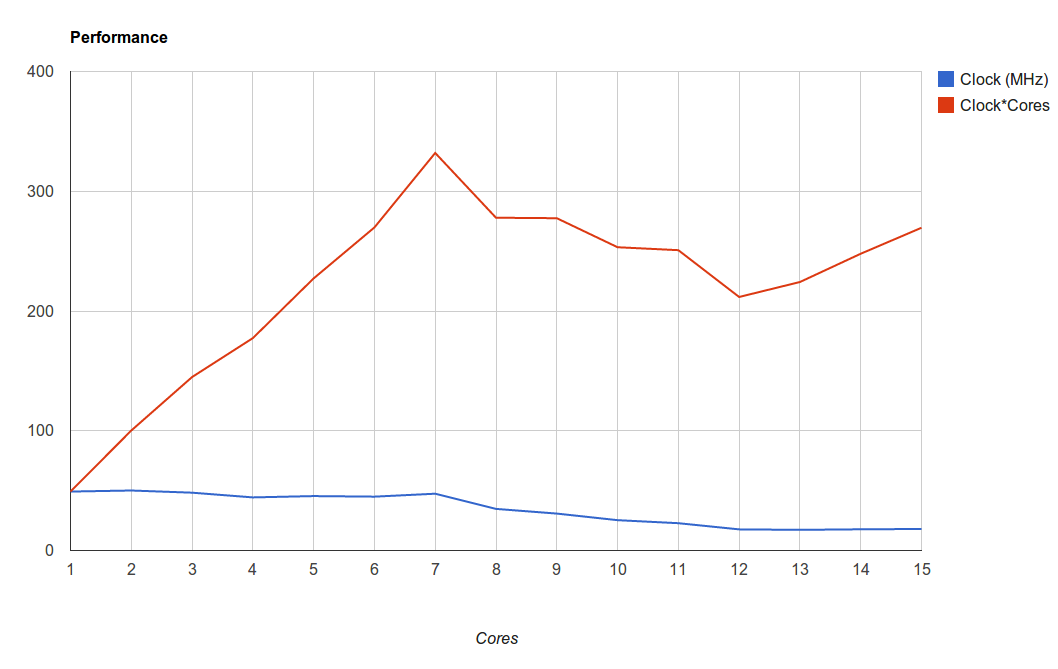
\includegraphics[width=\textwidth]{fpga/fig/performance.png}
    \caption{Total performance of Barricelli's fitness cores, as a function of number of cores}
    \label{figure:total-performance}
\end{figure}

The total performance of Barricelli's fitness cores, measured as maximum theoretical clock speed times number of clock cores, is illustrated in Figure \vref{figure:total-performance}.
This 

\todo{measure performance with different core amounts}

\todo{measure performance with and without genetics pipeline}

\todo{measure performance of same problems on consumer grade laptop}

\todo{measure performance of general program}



\section{Demonstration Programs}

This section documents the demonstration programs written for the Barricelli computer to demonstrate its functionality.
The programs are typically written in \gls{galapagos} assembly for programs running on the custom processor, and C for programs running on the \Gls{SCU}.
The source code for these demonstration programs can be found in appendix \vref{appendix:demonstration-programs-source-code}.

\subsection{Genetic Algorithm: Color Search}

The color search program is a very simple program demonstrating a basic usage of the genetics accelerator.
The program tries to find a specific color in the search-space of all 24-bit colors.

\subsubsection{Individual representation}

An individual represents a specific 24-bit color in RGB format.
The individual is coded to a 64-bit data word like in figure \vref{figure:color-search-bytefield}.

\begin{figure}[H]
    \begin{center}
        \begin{bytefield}[bitwidth=0.5em,endianness=big]{64}
            \bitheader[bitformatting={\tiny\rotatebox[origin=B]{90}}]{0, 7, 8, 15, 16, 23, 24, 63} \\
        \bitbox{40}{\color{lightgray}\rule{\width}{\height}}
            \bitbox{8}{blue}
            \bitbox{8}{green}
            \bitbox{8}{red}
        \end{bytefield}
        \caption{The binary coding of an individual for the color search problem}
        \label{figure:color-search-bytefield}
    \end{center}
\end{figure}

\subsubsection{Fitness Function}

The fitness for an individual is calculated using equation \vref{equation:color-search-fitness-function}.
The fitness a any given individual falls in the range $ [0, 768] $.

\begin{eqnarray}
\nonumber
fitness & = & 768 \\
\nonumber
        & - & |red_{individual} - red_{target}| \\
\nonumber
        & - & |green_{individual} - green_{target}| \\
        & - & |blue_{individual} - blue_{target}|
\label{equation:color-search-fitness-function}
\end{eqnarray}

\subsubsection{Results}

Figure \vref{figure:color-search} shows the evolution of the approximation suggested as an answer by the genetic algorithm.
In this problem instance the target color was magic pink, i.e. the color with color code $ rgb(255, 0, 255) $.
The program run illustrated in figure \vref{figure:color-search} ran on 7 seven cores, and the measurements are from regularly polling a single core for its current best solution.
Figure \vref{figure:color-search} clearly illustrates a typical trait of genetic algorithm approximations: they are quite good at finding decent approximations, but iterating to improve accuracy of the result is a game of diminishing returns.
The algorithm quickly finds a decent approximation of the target color, but finding the exact value down to the last bit still takes time.

\begin{figure}[H]
    \begin{center}
        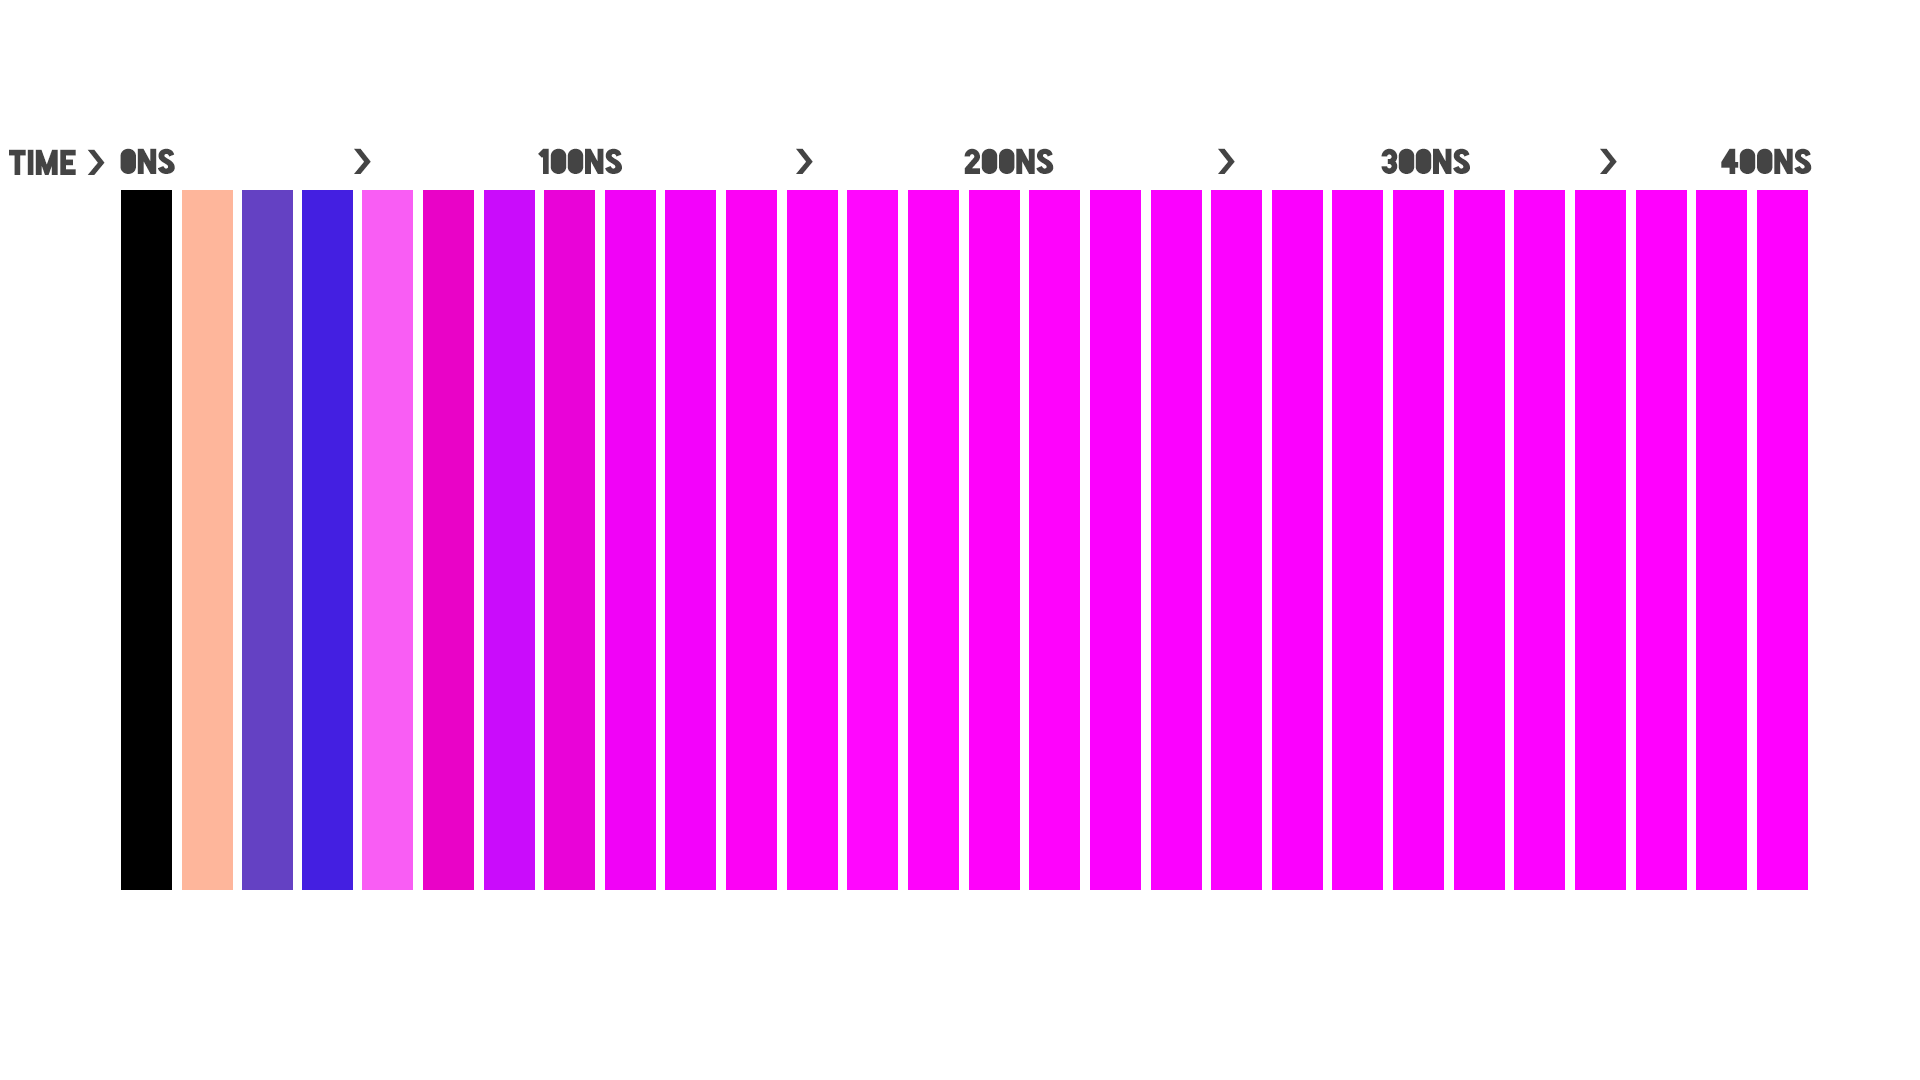
\includegraphics[width=\textwidth]{fig/color-search}
    \caption{Color search progression (7 cores, 1 core sampled)}
    \label{figure:color-search}
    \end{center}
\end{figure}

\subsection{Genetic Algorithm: Binary Knapsack Problem}

The knapsack problem is an optimization problem that is considered NP-hard.
The problem to solve is given a set of items with a weight and a value and a knapsack that can hold a specific weight, what combination of items that can fit in the sack has the highest value.
If there can be at most one of each item in the knapsack, we have what is known as the binary knapsack problem.

\subsubsection{Individual representation}

An individual represents a combination of items.
The individual is coded to a 64-bit data word like in Figure \vref{figure:binary-knapsack-bytefield}.

\begin{figure}[H]
    \begin{center}
        \begin{bytefield}[bitwidth=0.5em,endianness=big]{64}
            \bitheader{0, 63} \\
            \bitbox{63}{bit $ i $ set if item $ i $ is in the include set, else unset}
        \end{bytefield}
        \caption{The binary coding of an individual for the binary knapsack problem}
        \label{figure:binary-knapsack-bytefield}
    \end{center}
\end{figure}

\subsubsection{Fitness Function}
The fitness for an individual is calculated using Algorithm \ref{algorithm:binary-knapsack-fitness-function}.
The fitness falls between 0 for invalid sacks (that contain too much weight) to a theoretical maximum of the sum of the value of all the items.

\begin{algorithm}[H]
\SetAlgoLined
\DontPrintSemicolon
\KwData{A bit array with one bit representing whether each item is included or not}
\KwResult{How fit the individual is}
\Begin{
    $ weight \longleftarrow 0$\;
    $ value \longleftarrow 0$\;
    \For {item in ItemSet} {
        \If {item in genome} {
            $ weight \longleftarrow weight + item.weight$\;
            $ value \longleftarrow value + item.value$\;

            \If {$weight > maxWeight$} {
                $ value \longleftarrow 0$\;
                $ break $\;
            }
        }
    }
    \;
    \Return{$ value $}
}
\caption{The fitness function for the binary knapsack problem}
\label{algorithm:binary-knapsack-fitness-function}
\end{algorithm}

\subsubsection{Results}

This problem has not been run on the actual hardware, only simulated up to a few milliseconds.
The simulation seemed fine, and we got increasing fitness values, but the problem space is huge, so we probably need to run the algorithm for quite some time before coverging to a ideal/near-ideal solution.

\subsection{Blinkenlights}
Blinkenlights is a program that demonstrates the use of the input and output of the \Gls{barricelli} driven by the \Gls{SCU}.
When a button is pressed, the corrensponding LEDs to the button lit up.
This program is also described as a test for I/O, in \vref{iotest}, named Buttons \& LEDs.



\section{Discussion}
	\section{Performance}

The Barricelli computer is designed to be a device for high performance parallel computing.
Throughout the design process, choices have been made that further this goal.

The computer architecture is capable of executing multiple independent instruction streams working on multiple different independent data streams, which means that parallelism can be exploited to a large degree to achieve a high computational throughput.
A heterogenic collection of cores, some general, and some working as specialized accelerators, combines the allround-ness and usability of general computing with the at times extreme performance boosts given by specialized workers.

The general cores have been designed to exploit instruction-level parallelism, iwth features such as pipelining, hazard detection and correction using forwarding, and branch prediction.

The intelligent off-line assembler also helps off-load some of the hazard detection work from the processor, which lets the processor spend more of its valuable time computing.

Since the computer uses a shared memory bus though a single memory controller, it is an obvious scalability limitor.
For the instruction memory, this is somewhat mitigated by the inclusion of instruction caches, but there is still room for improvement.
To improve the memory performance, memory could be organized in a more hierarchical fashion, with multiple cache levels.

\subsection{Performance Measurements and Benchmarking}

With the specified prototype of the Barricelli computer presented in this report, looking at the results from the performance measurements in Chapter \vref{chapter:tests}, the optimal number of parallel fitness cores is 7.
Up to 7 processors, the performance scales beautifully, with calculated total performance scaling linearly with the number of cores.
After 7 cores, the relative performance of each core drops.
It is not easy to see exactly why this happens, but it is quite probably related to resource usage of the FPGA.

As the number of fitness cores increases, the more pressure it puts on the genetics accelerator.
As the number of fitness cores increases, the number of accelerators should also increase.

\subsection{Average Instructions per Cycle}

In optimal condititons, i.e.
the pipeline is filled, and no register spilling occurs, the processor can execute $ n $ instructions per cycle, where $ n $ is the number of processors.
In the designed protoype of Barricelli, this means that the maximum instructions per second is $ 7 cores * 50Mhz = 350 000 000 $, or 350 Mega-instructions per second.

\section{Theory}
In this section theory related to MIMD architectures and how to further improve their performances are discussed.
This also covers the discussions inside the group about the design of the architecture in the planning phase of the project.
\subsection{SPMD and Concurrency}
One of the first discussions that came up in the group after the assignment were given was if the processor cores should
be able to synchronize themselves.
By doing this, the processor cores would be able to execute code that is not completely independent in parallel in an elegant way.
However this also raises some issues as for instance data hazards.


\subsection{Using CISC or RISC ISAs}
CISC and RISC instruction set architectures are two very different ways of thinking when it comes to creating instruction sets.
While in the last years, RISC ISAs have been the most dominant instruction set architecture, we can also see that CISC architectures
are on their way back into the markets.
Some of the reasons for this is that increasing parallelism is gaining lesser performance increases.

\subsubsection{Micro Operations: a Bridge Between Complex and Reduced Instruction Sets}
The use of micro operations is based on the principle that you want to convert a complex instruction into a set of smaller micro operations.
This
may simplify the design of for instance a super scalar processor because dependencies between the converted micro instructions would already be known.


\subsection{Memory Management Policies}

The Galapagos architecture operates with several types of shared memory: \emph{instruction memory}, \emph{data memory}, \emph{instruction caches}, \emph{rated pool} and \emph{unrated pool}.
These types of memories  can further be divided into two groups: memory and genetic related.
These two groups are connected to separate data and address buses.
The access to these buses are handled by a request-acknowledgement protocol.
The responsible of this protocol is to control the access to the shared memories and their respective buses.
The protocol is based in the ideas of round-robin scheduling.
The request lines are continuously polled by the controllers in a round-robin fashion.
The reason for choosing this algorithm is because it is considered to be fair.
Since each request line is checked in turn, the algorithm is considered starvation free.
A requesting core will eventually get its request handled by the controllers.


Since all the cores access the same memories this solution will, however, turn out to be quite slow.
Note that every core is in fact competing for the access to memory.
For memory intensive problems this bottleneck will be quite visible.
Every time cores wishes to perform simultaneously some memory access only one of them will be granted access.
For instance, consider a system with five cores.
If these cores have a relatively frequent memory access pattern it pretty self explanatory that this will cause the the different cores being idle most of the time.
This will imply that the memory scheme in the galapagos architecture does not scale very well.
This implies that the more cores that are present the less performance would be achieved.


A possible solution for this problem would have been keeping separate data caches for each core.
Then the cores could have been using the data located in the caches instead of accessing the memory so frequently.
When first accessing the memory, the core could have loaded several data elements instead of just one word for each request.
This would surely been an improvement for the memory system employed in the baracelli currently.
This would, however, been very difficult to achieve, and is not in the scoop of this assignment.
Private data caches would require implementing cache coherence algorithms for keeping the caches consistent.
This is considered very difficult.



\subsubsection{Cache Coherency}
MIMD architecture use a shared memory models.
This imposes a problem when using caches, and memory in general.
When more core updates on the same values on the same memory positions; memory collisions occur.
These problems can be fixed by enforcing that only one core is able to access the memory at any given time.
A far more difficult problem is the problem of cache coherence.
Cache coherency issues occurs when several cores have private caches containing the same data, and some core changes the data.
Then the data in the caches is not consistent among the cores.
In order for the data to be consistent, in this example, is for each core having the same data.
Note that same data in this context mean data from the same memory location.


The Galapagos architecture does not support private data caches.
This design choice relieves the processor designer of implementing advanced cache coherency algorithms in hardware.
Instead of private data caches the Galapagos architectures employ shared pools for rated and un-rated chromosomes.
These are connected to a bus and the connected through the \emph{genetic controller}.
The controller is configured to only allow one core perform its operation on one of the pools at any given time.
This implies that read and write operations are atomic.
As a direct consequence cache coherency issues are not possible in the architecture.


\part{Appendices}
	\appendix
\chapter{Galapagos Instruction Set Architecture Documentation} \label{appendix:isa}
\newpage
\includepdf[pages=-]{isa/isa.pdf}

\chapter{PCB schematics} \label{appendix:pcb-schematics}
\newpage

\chapter{Case schematics} \label{appendix:case-schematics}
\newpage

\chapter{Galapos Assembler Listing} \label{appendix:galapagos-assembler-source-code}
\newpage

\lstinputlisting[language=Python]{galapagos-assembler/galapagos/__init__.py}
\lstinputlisting[language=Python]{galapagos-assembler/galapagos/assembler.py}
\lstinputlisting[language=Python]{galapagos-assembler/galapagos/base.py}
\lstinputlisting[language=Python]{galapagos-assembler/galapagos/instructions.py}
\lstinputlisting[language=Python]{galapagos-assembler/galapagos/scanner.py}

\chapter{Demonstration Program Listings} \label{appendix:demonstration-programs-source-code}
\newpage

\chapter{Budget} \label{appendix:budget}
\newpage


\bibliography{reference-library}
\bibliographystyle{plain}
\nocite{*}

\end{document}